%---------------------------------------------
% Lachaise Assignment
% LaTeX Template
% Version 1.0 (26/6/2018)
%
% This template originates from:
% http://www.LaTeXTemplates.com
%
% Authors:
% Marion Lachaise & François Févotte
% Vel (vel@LaTeXTemplates.com)
%
% License:
% CC BY-NC-SA 3.0 (http://creativecommons.org/licenses/by-nc-sa/3.0/)
% 
%---------------------------------------------------

%----------------------------------------------------------------------------------------
%	PACKAGES AND OTHER DOCUMENT CONFIGURATIONS
%----------------------------------------------------------------------------------------

\documentclass{article}
% Include the file specifying the document structure and custom commands
%%%%%%%%%%%%%%%%%%%%%%%%%%%%%%%%%%%%%%%%%
% Lachaise Assignment
% Structure Specification File
% Version 1.0 (26/6/2018)
%
% This template originates from:
% http://www.LaTeXTemplates.com
%
% Authors:
% Marion Lachaise & François Févotte
% Vel (vel@LaTeXTemplates.com)
%
% License:
% CC BY-NC-SA 3.0 (http://creativecommons.org/licenses/by-nc-sa/3.0/)
% 
%%%%%%%%%%%%%%%%%%%%%%%%%%%%%%%%%%%%%%%%%

%----------------------------------------------------------------------------------------
%	PACKAGES AND OTHER DOCUMENT CONFIGURATIONS
%----------------------------------------------------------------------------------------

\usepackage[ngerman]{babel} %UMLAUTE

\usepackage{amsmath,amsfonts,stmaryrd,amssymb} % Math packages

\usepackage{enumerate} % Custom item numbers for enumerations

\usepackage[ruled]{algorithm2e} % Algorithms

\usepackage[framemethod=tikz]{mdframed} % Allows defining custom boxed/framed environments

\usepackage{listings} % File listings, with syntax highlighting
\lstset{
	basicstyle=\ttfamily, % Typeset listings in monospace font
}

\usepackage{graphicx}
%Path relative to the main .tex file 
\graphicspath{ {images/} }

%----------------------------------------------------------------------------------------
%	DOCUMENT MARGINS
%----------------------------------------------------------------------------------------

\usepackage{geometry} % Required for adjusting page dimensions and margins

\geometry{
	paper=a4paper, % Paper size, change to letterpaper for US letter size
	top=2.5cm, % Top margin
	bottom=3cm, % Bottom margin
	left=2.5cm, % Left margin
	right=2.5cm, % Right margin
	headheight=14pt, % Header height
	footskip=1.5cm, % Space from the bottom margin to the baseline of the footer
	headsep=1.2cm, % Space from the top margin to the baseline of the header
	%showframe, % Uncomment to show how the type block is set on the page
}

%----------------------------------------------------------------------------------------
%	FONTS
%----------------------------------------------------------------------------------------

\usepackage[utf8]{inputenc} % Required for inputting international characters
\usepackage[T1]{fontenc} % Output font encoding for international characters

\usepackage{XCharter} % Use the XCharter fonts

%----------------------------------------------------------------------------------------
%	COMMAND LINE ENVIRONMENT
%----------------------------------------------------------------------------------------

% Usage:
% \begin{commandline}
%	\begin{verbatim}
%		$ ls
%		
%		Applications	Desktop	...
%	\end{verbatim}
% \end{commandline}

\mdfdefinestyle{commandline}{
	leftmargin=10pt,
	rightmargin=10pt,
	innerleftmargin=15pt,
	middlelinecolor=black!50!white,
	middlelinewidth=2pt,
	frametitlerule=false,
	backgroundcolor=black!5!white,
	frametitle={Command Line},
	frametitlefont={\normalfont\sffamily\color{white}\hspace{-1em}},
	frametitlebackgroundcolor=black!50!white,
	nobreak,
}

% Define a custom environment for command-line snapshots
\newenvironment{commandline}{
	\medskip
	\begin{mdframed}[style=commandline]
}{
	\end{mdframed}
	\medskip
}

%----------------------------------------------------------------------------------------
%	FILE CONTENTS ENVIRONMENT
%----------------------------------------------------------------------------------------

% Usage:
% \begin{file}[optional filename, defaults to "File"]
%	File contents, for example, with a listings environment
% \end{file}

\mdfdefinestyle{file}{
	innertopmargin=1.6\baselineskip,
	innerbottommargin=0.8\baselineskip,
	topline=false, bottomline=false,
	leftline=false, rightline=false,
	leftmargin=2cm,
	rightmargin=2cm,
	singleextra={%
		\draw[fill=black!10!white](P)++(0,-1.2em)rectangle(P-|O);
		\node[anchor=north west]
		at(P-|O){\ttfamily\mdfilename};
		%
		\def\l{3em}
		\draw(O-|P)++(-\l,0)--++(\l,\l)--(P)--(P-|O)--(O)--cycle;
		\draw(O-|P)++(-\l,0)--++(0,\l)--++(\l,0);
	},
	nobreak,
}

% Define a custom environment for file contents
\newenvironment{file}[1][File]{ % Set the default filename to "File"
	\medskip
	\newcommand{\mdfilename}{#1}
	\begin{mdframed}[style=file]
}{
	\end{mdframed}
	\medskip
}

%----------------------------------------------------------------------------------------
%	NUMBERED QUESTIONS ENVIRONMENT
%----------------------------------------------------------------------------------------

% Usage:
% \begin{question}[optional title]
%	Question contents
% \end{question}

\mdfdefinestyle{question}{
	innertopmargin=1.2\baselineskip,
	innerbottommargin=0.8\baselineskip,
	roundcorner=5pt,
	nobreak,
	singleextra={%
		\draw(P-|O)node[xshift=1em,anchor=west,fill=white,draw,rounded corners=5pt]{%
		Question \theQuestion\questionTitle};
	},
}

\newcounter{Question} % Stores the current question number that gets iterated with each new question

% Define a custom environment for numbered questions
\newenvironment{question}[1][\unskip]{
	\bigskip
	\stepcounter{Question}
	\newcommand{\questionTitle}{~#1}
	\begin{mdframed}[style=question]
}{
	\end{mdframed}
	\medskip
}

%----------------------------------------------------------------------------------------
%	WARNING TEXT ENVIRONMENT
%----------------------------------------------------------------------------------------

% Usage:
% \begin{warn}[optional title, defaults to "Warning:"]
%	Contents
% \end{warn}

\mdfdefinestyle{warning}{
	topline=false, bottomline=false,
	leftline=false, rightline=false,
	nobreak,
	singleextra={%
		\draw(P-|O)++(-0.5em,0)node(tmp1){};
		\draw(P-|O)++(0.5em,0)node(tmp2){};
		\fill[black,rotate around={45:(P-|O)}](tmp1)rectangle(tmp2);
		\node at(P-|O){\color{white}\scriptsize\bf !};
		\draw[very thick](P-|O)++(0,-1em)--(O);%--(O-|P);
	}
}

% Define a custom environment for warning text
\newenvironment{warn}[1][Warning:]{ % Set the default warning to "Warning:"
	\medskip
	\begin{mdframed}[style=warning]
		\noindent{\textbf{#1}}
}{
	\end{mdframed}
}

%----------------------------------------------------------------------------------------
%	INFORMATION ENVIRONMENT
%----------------------------------------------------------------------------------------

% Usage:
% \begin{info}[optional title, defaults to "Info:"]
% 	contents
% 	\end{info}

\mdfdefinestyle{info}{%
	topline=false, bottomline=false,
	leftline=false, rightline=false,
	nobreak,
	singleextra={%
		\fill[black](P-|O)circle[radius=0.4em];
		\node at(P-|O){\color{white}\scriptsize\bf i};
		\draw[very thick](P-|O)++(0,-0.8em)--(O);%--(O-|P);
	}
}

% Define a custom environment for information
\newenvironment{info}[1][Info:]{ % Set the default title to "Info:"
	\medskip
	\begin{mdframed}[style=info]
		\noindent{\textbf{#1}}
}{
	\end{mdframed}
}
 
\usepackage{hyperref}
\usepackage[utf8]{inputenc}
\usepackage{caption}
%----------------------------------------------------------------------------------------
%	INFORMATION
%----------------------------------------------------------------------------------------

% Title
\title{Open Source Roboter Plattform} 

\author{Lukas Reichwein\\ Yves Ehrlich\\ Nick Gnoevoj}

\date{University of Applied Science Fulda --- \today} 

%----------------------------------------------------------------------------------------

\begin{document}

\maketitle % Print the title
\tableofcontents % Inhaltsverzeichniss, Achtung zweimal Compilerien!
%\newpage

%----------------------------------------------------------------------------------------
%	INTRODUCTION
%----------------------------------------------------------------------------------------

\section{Vorwort} % Unnumbered section
    \paragraph{Motivation: }
    Eine Plattform bieten ist etwas, das momentan sehr stark im Trend liegt, sei es im Software oder im Hardware Bereich. Im Softwarebereich zeigt sich dies meist durch Open-Source Bibliotheken, welche möglichst variabel einsetzbaren Code für jeden frei zugänglich machen.    
    Ein solches Projekt war auch von einem der Projektmitglieder (Yves Ehrlich) als Privates Projekt geplant und so kam die Überlegung dies innerhalb des Modules Embedded Networking zu wählen.
    \paragraph{Basis des Projektes: }
    Als Basis des Projektes dient einer schon bereits von Yves Ehrlich angefertigter Arduino Nano Shield samt Code,
    \cite{nanoGame} welcher als Fernsteuerung verwendet wird. 
    \paragraph{Ziel des Projektes: }	
	Ziel des Projektes ist ein ferngesteuerte, Open-Source basierende Roboterplattform.

\newpage    
\section{Überlegung}%Yves

Die urprüngliche Idee war die Entwicklung eines Solarroboters, also eines Roboters, der tagsüber mit Hilfe der Sonneneinstrahlung seinen Eigenbedarf decken kann und somit nur einen kleinen Pufferakku benötigt.
Praktische Anwendungen könnten z.B. die Nutzung als kompakte Straßenkehrmaschine oder als Rasenmäher sein. Bedingt durch die eingeschränkte Leistungsabgabe der Solarzellen vermutlich nur für kleine zu bearbeitende Flächen.
Da es nur wenige brauchbare und frei zugängliche Quellen für solche Plattformen gibt, wollten wir eine eigene schaffen. Daher sollte das Projekt exemplarisch als Grundlage für eine Quelloffene Plattform dienen, die auch von anderen genutzt und weiterentwickelt werden kann.

Da wir bei der Entwicklung der mechanischen Komponenten schnell feststellen mussten, dass das Fahrwerk recht komplex ist, insbesondere die Vorderachse, schwenkten wir schnell auf eine andere Bauweise um. Zunächst war der Aufbau mit 4 gleichen Rädern geplant, von denen zwei Stück (Hinterachse) von einem bürstenlosen Gleichstrommotor angetrieben werden sollten. Die Entwicklung eines Differenzials gestaltete sich noch als relativ einfach. Die Vorderachse aber mit dem Servo gestaltete sich dann, hinsichtlich des Zeitaufwandes, für zu komplex.

\begin{figure}[h]
	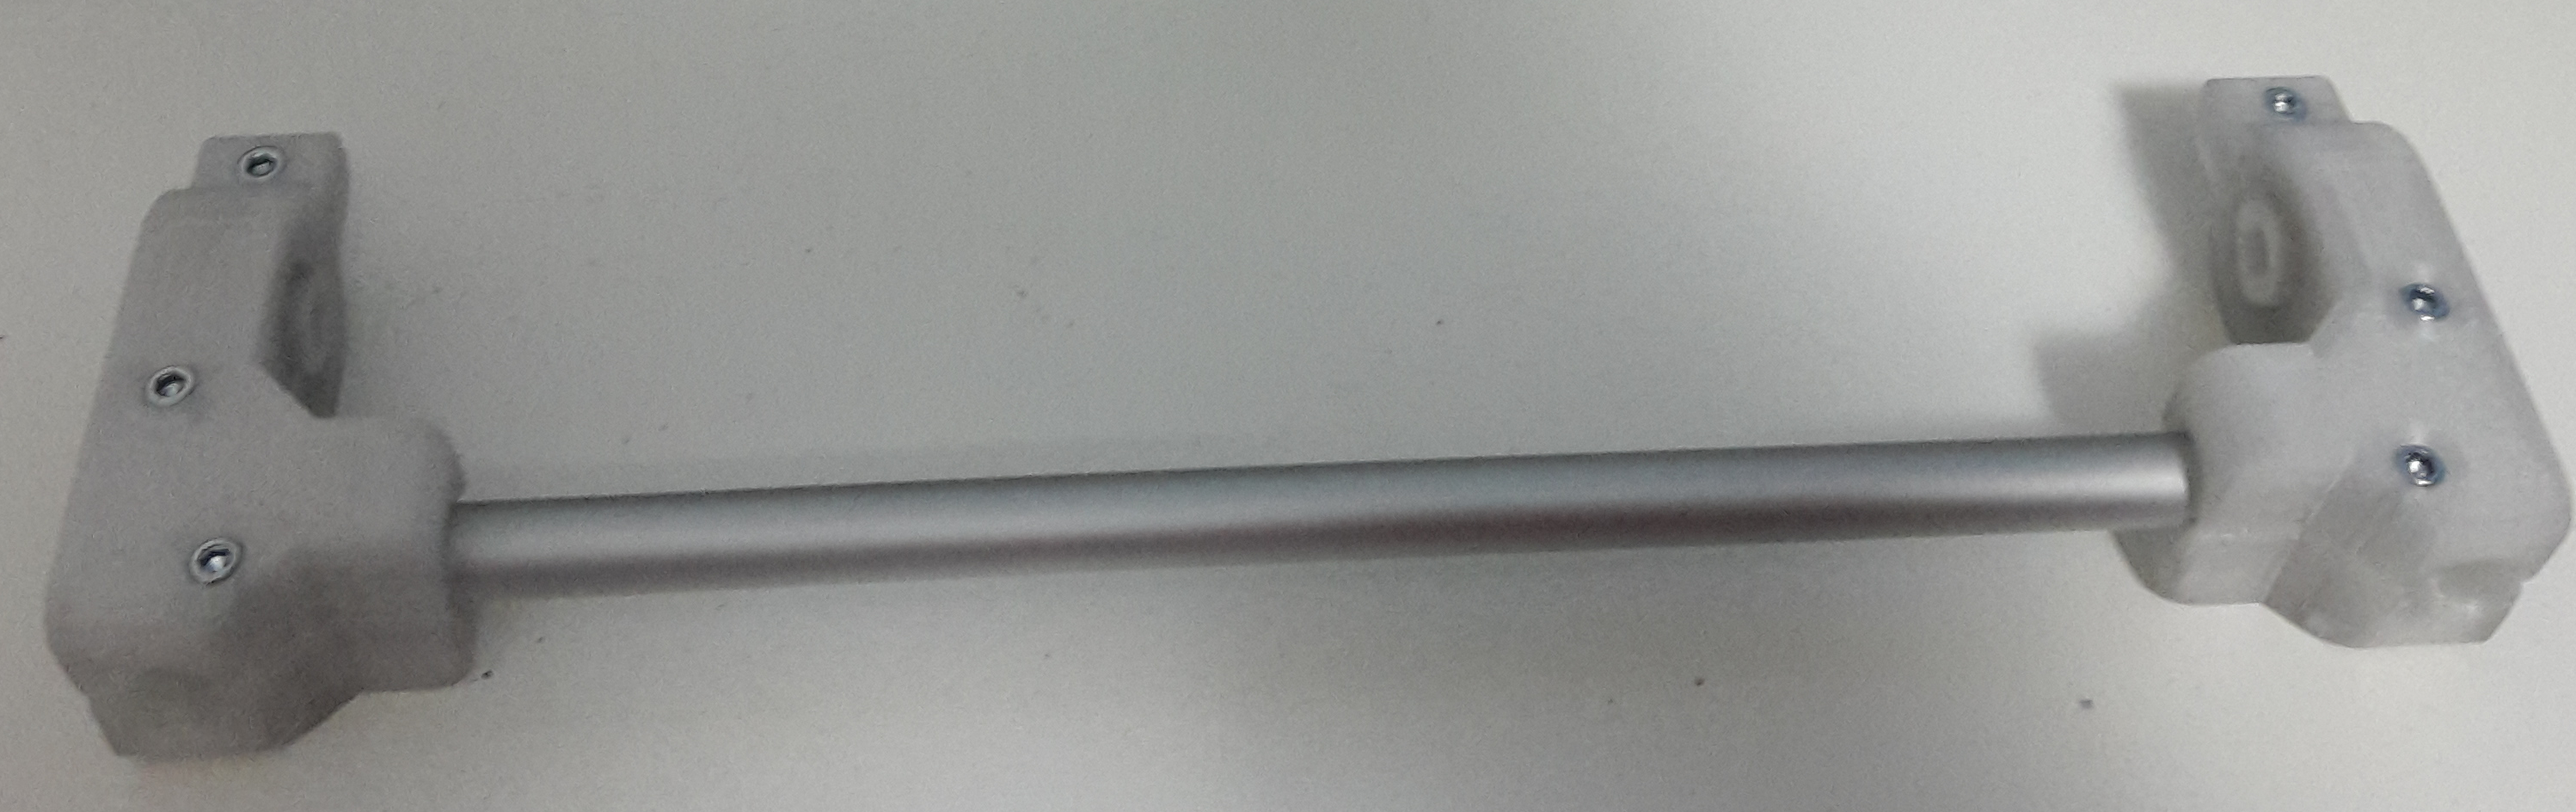
\includegraphics[width=12cm]{hinterachse.png}
	\centering
	\caption{Hinterachse des urpsrünglichen Aufbaus}
\end{figure}

\begin{figure}[h]
	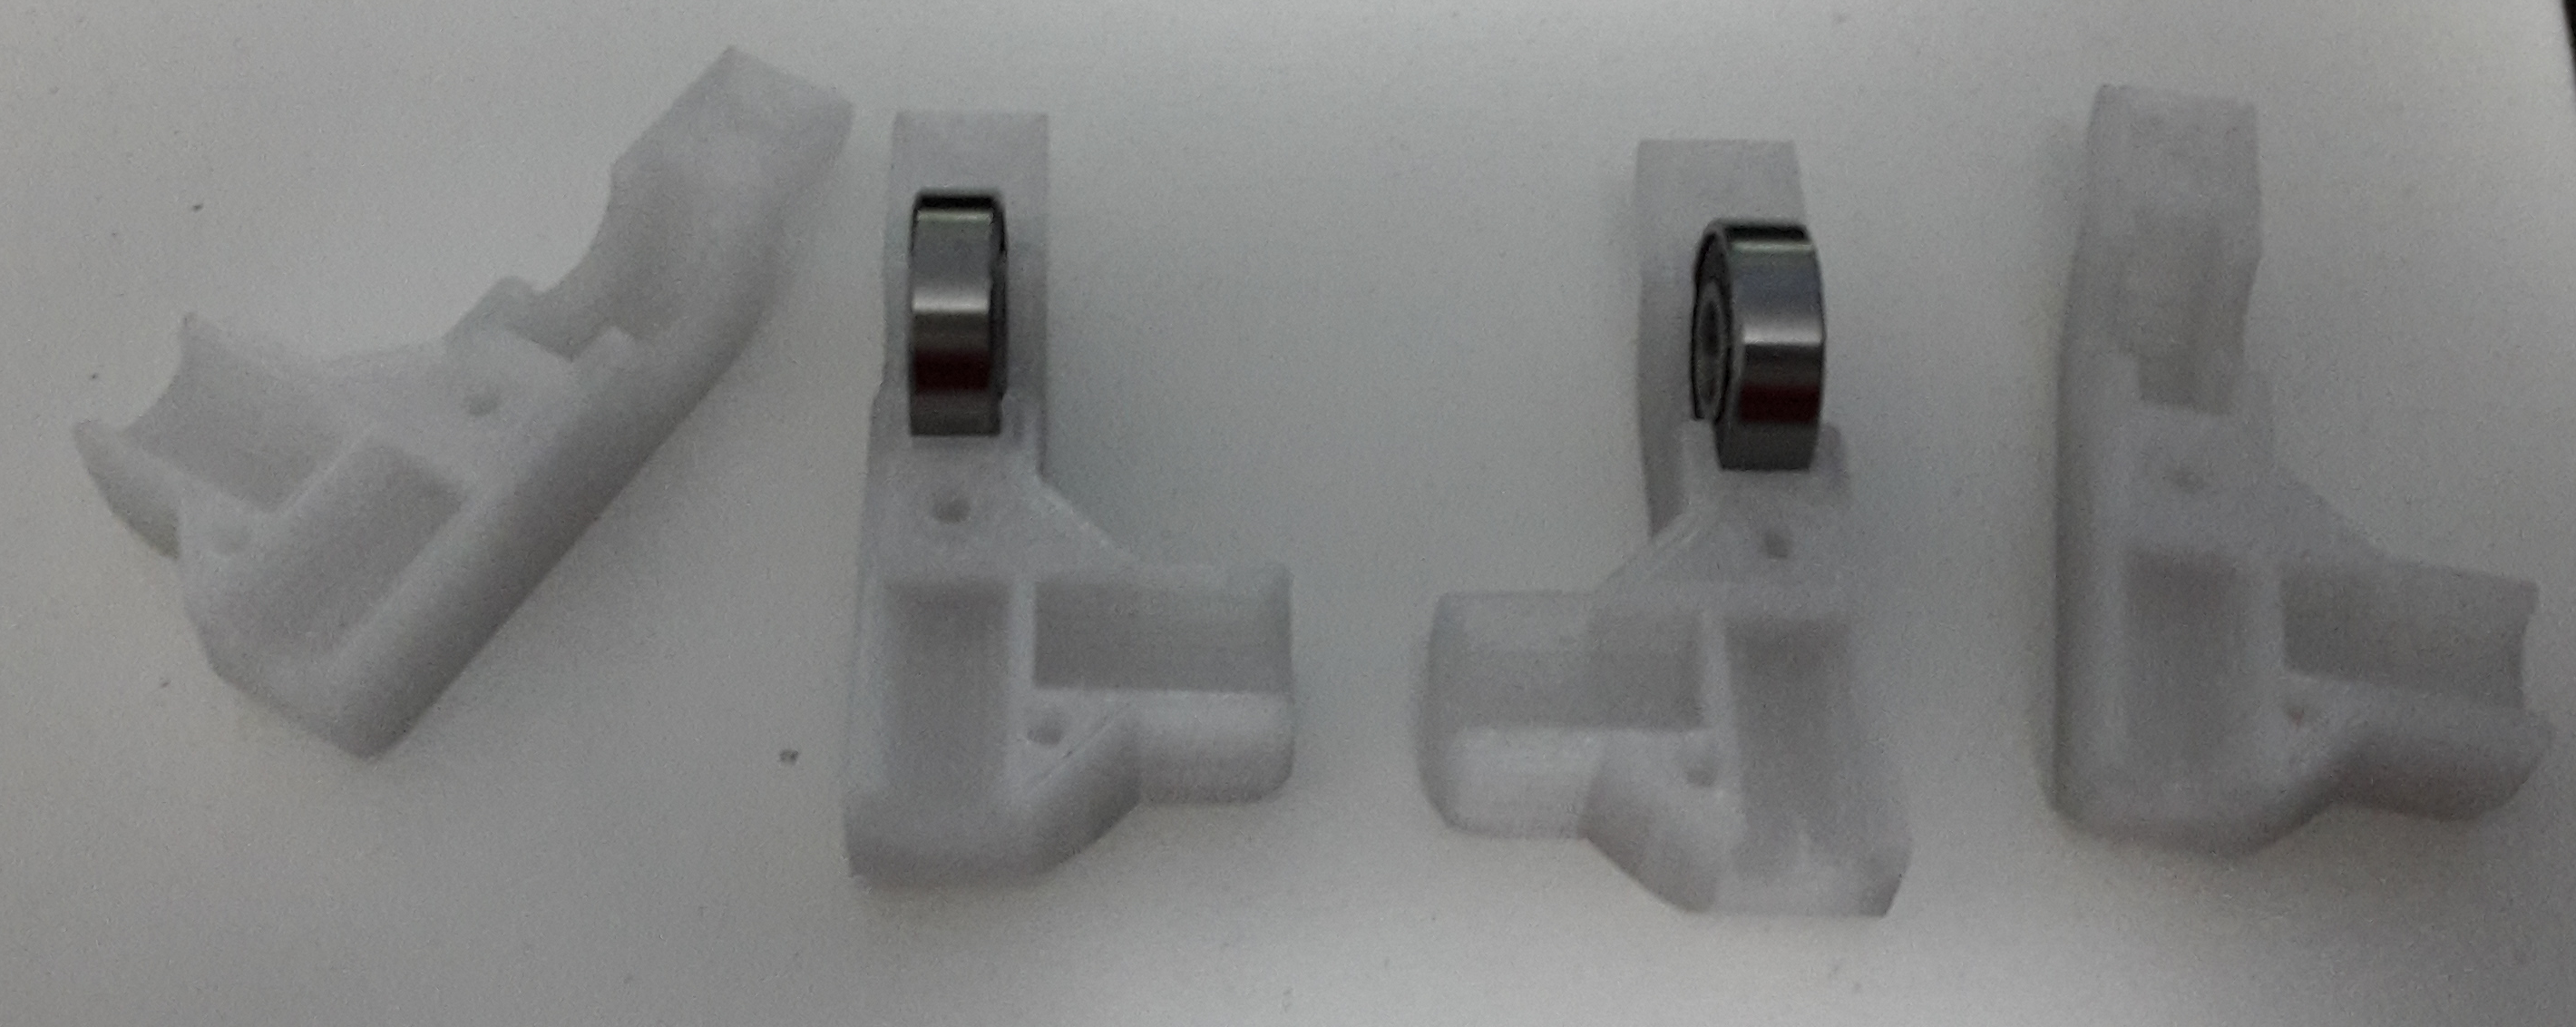
\includegraphics[width=12cm]{lagerschalen.png}
	\centering
	\caption{Lagerschalen}
\end{figure}

Somit schwenkten wir kurzer Hand zu einem sehr viel einfacheren Aufbau um, um uns schneller den wichtigeren Komponenten widmen zu können.
Der neue Aufbau sah eine schlichte Grundplatte als Plattform für die weiteren Bauteile, wie Motoren (Mabuchi N20 mit Getriebe), Ultraschallsensor, Akku, Hauptplatine und uvm. vor.
Um möglichst viele Montagemöglichkeiten zu bieten, wurde die Grundplatte mit Bohrungen in regelmäßigen Abständen versehen. Diese Bohrungen können zum durchstecken für Schrauben oder zum versenken von Gewindemuffen genutzt werden.
Zum anbringen unserer Komponenten haben wir auf Messinggewindebuchsen und passende M3 Schrauben gesetzt.
Alle selbstentworfenen Komponenten haben wir mit einem FFF 3D-Drucker aus PLA gedruckt.
Mit Ausnahme der Hauptplatine natürlich.
Bedingt durch den Zeitaufwand des gesamten Projektes und anderer Studienmodule haben wir uns entschieden, die Implementierung eines MPPT Ladereglers fallen zu lassen, somit wurde die Idee des Solarroboters auf die Idee der Entwicklung eines Roboters reduziert.

\begin{figure}[h]
	\includegraphics[width=12cm]{roboter.png}
	\centering
	\caption{Der Roboter, aktueller Aufbau}
\end{figure}

\newpage    
\section{Mechanik}%Yves

Wie bereits unter „Überlegung“ erwähnt, gestaltete sich der Aufbau mit Achsträger, Radlager und Lagerschalen uvm. als zu Zeitintensiv um in der vorgegebenen Zeit bewältig werden zu können.
Zum Entwurf der mechanischen Bauteile wurde das CAD Programm Fusion 360 von Autodesk verwendet. Dabei gab es kaum Schwierigkeiten, da Yves Ehrlich bereits sehr viel Erfahrung mit 3D-CAD Programmen gesammelt hat. Lediglich der Zwang Windows zu benutzen stellt eine ständige Unannehmlichkeit dar.

Alle Entwürfe wurden mit einem 3D Drucker gedruckt, einem HCmaker7, ein Klon des bekannten Creality CR-10S.
Das Material der Wahl war PLA. Für einen Außeneinsatz ist das Material wegen der geringen Witterungsbeständigkeit kaum geeignet. Insbesondere die geringe Temperaturbeständigkeit (max. 60°C) disqualifizieren das Material für den Einsatz in der Sonne. Da dies aber ohnehin nicht mehr geplant war, ist das Material für unseren Zweck geeignet.
\subsection{Montagemöglichkeiten}
Die zur Befestigung von Bauteilen nötigen Gewindebuchsen in den Kunststoff einzusetzen ist relativ einfach, man benötigt dafür lediglich eine Schraube die man in die Buchse einschraubt und einen Lötkolben mit einer Temperatur von etwa 240°C. Ohne Druck auszuüben legt man die Spitze des Lötkolbens auf den Schraubenkopf. Wenn die Schraube ausreichend Wärme an die Muffe übertragen hat, fängt die Muffe an im Kunststoff zu versinken. Die Schwerkraft sorgt hier für alles nötige. Wenn die Muffe weit genug versunken ist, kann der Lötkolben entfernt werden und man sollte die Schraube schnell abkühlen, z.B. durch pusten oder ein kleines Gebläse wie z.B. einen Radiallüfter.
Beim Design der Kunststoffteile muss man darauf achten, dass für Gewindemuffen stehts eine ausreichend große Fase vorhanden sein muss, damit die Muffe einerseits zentriert wird beim versinken und andererseits kein verdrängtes Material die Muffe beim versinken behindert oder verstopft. Letzterem wird aber auch durch die eingeschraubte Schraube vorgebeugt.
\subsection{Antrieb}
Der Aufbau sieht zwei Antriebsmotoren vor, welche jeweils ein Rad treiben. Zum abstützen verfügt der Roboter über ein selbstentworfenes Kugelrad. Dieses Kugelrad verwendet als Kugeln vier handelsübliche Airsoft Kugeln mit einem Durchmesser von 6mm.
Die Gleiteigenschaften dieser Konstruktion sind nicht die besten, aber für diesen Prototypen ausreichend. Um die Reibung zu vermindern haben wir Silikonöl auf die Kugeln aufgetragen.
\subsection{Verbesserung}
Da Kunststoffe auf glatten Oberflächen sehr wenig Bodenhaftung haben, wurden die Räder mit einer Nut versehen. In diese Nut kann man später ein einfaches Haushaltsgummiband einlegen, somit hat der Roboter auch auf glatten Oberflächen relativ gute Haftung.

\newpage    
\section{Elektronik}%Yves

Lochrasterplatinen, wie sie häufig für Prototypzwecke genutzt werden, sind nicht nur unpraktisch für SMD Komponenten, auch wenn man ein 2,54mm Raster mit einigen Tricksereien durchaus auch für SMD Komponenten nutzen kann, sie sind auch relativ unzuverlässig und die Fehlersuche gestaltet sich z.T. als schwierig (je nach Menge und Komplexität der Verdrahtungslagen).
Deshalb entschieden wir uns, eine eigene Platine zu entwickeln.
Als Software nutzten wir dafür das kommerzielle Programm Sprint Layout 6 von der Firma Abacom.

Da die Herstellung der Platine von Hand erfolgen sollte, haben wir die Strukturen der Platine sehr grob gezeichnet. Was auch durch die geringe Anzahl an Komponenten und deren modulare Bauweise begünstigt wurde.

\subsection{Verfahren}%Yves

Als Verfahren zum beschichten der Platine diente die Tonertransfermethode. Dabei wird die Schaltung mit einem Laserdrucker auf geeignetes Papier gedruckt, in diesem Fall Photopapier, und dann mit Hitze auf die blanke Platine gedrückt. Für diesen Zweck hat Yves Ehrlich ein Laminiergerät umgebaut, welches den Vorgang erheblich erleichtert.
Da unsere Platine doppelseitig ist, müssen zuvor die zwei Seiten, welche die Schaltung enthalten Deckungsgleich aufeinander ausgerichtet werden und dann an den Rändern verklebt werden, damit man am Ende eine Art Tasche erhält, in welche dann die Platine eingesteckt werden kann.
Das ganze läuft dann einige Male durch das Laminiergerät. Nach dem das erfolgt ist, lässt man die Platine etwas abkühlen und ab einer Temperatur von etwa 30-40°C schneidet man die Tasche seitlich auf und zieht vorsichtig das Papier ab. Der Toner bleibt am Kupfer haften und schützt an diesen Stellen, wie ein Fotolack, das Kupfer davor weggeätzt zu werden.
Anschließen gibt man die beschichtete Platine in eine Ätzküvette welche mit einer Natriumpersulfat-Lösung gefüllt ist. Nach einiger Zeit kann man beim durchleuchten der Küvette sehen, wie sich das Kupfer immer weiter auflöst, bis am Ende die Schaltung klar und deutlich zu sehen ist. Dann wird die Platine entnommen und gründlich mit Wasser abgespült.
Zum entfernen des Toners benötigt man etwas Aceton und einen Lappen.
Für die THT Komponenten müssen nun noch Bohrungen gesetzt werden. 1,2mm, passend für die Durchkontaktiernieten von Bungard.
Nach dem verpressen (mangels passender Presse eher mit einem Körner breitschlagen) der Nieten, müssen diese beidseitig verlötet werden. Danach können alle Komponenten bestückt werden.

\begin{figure}[h]
	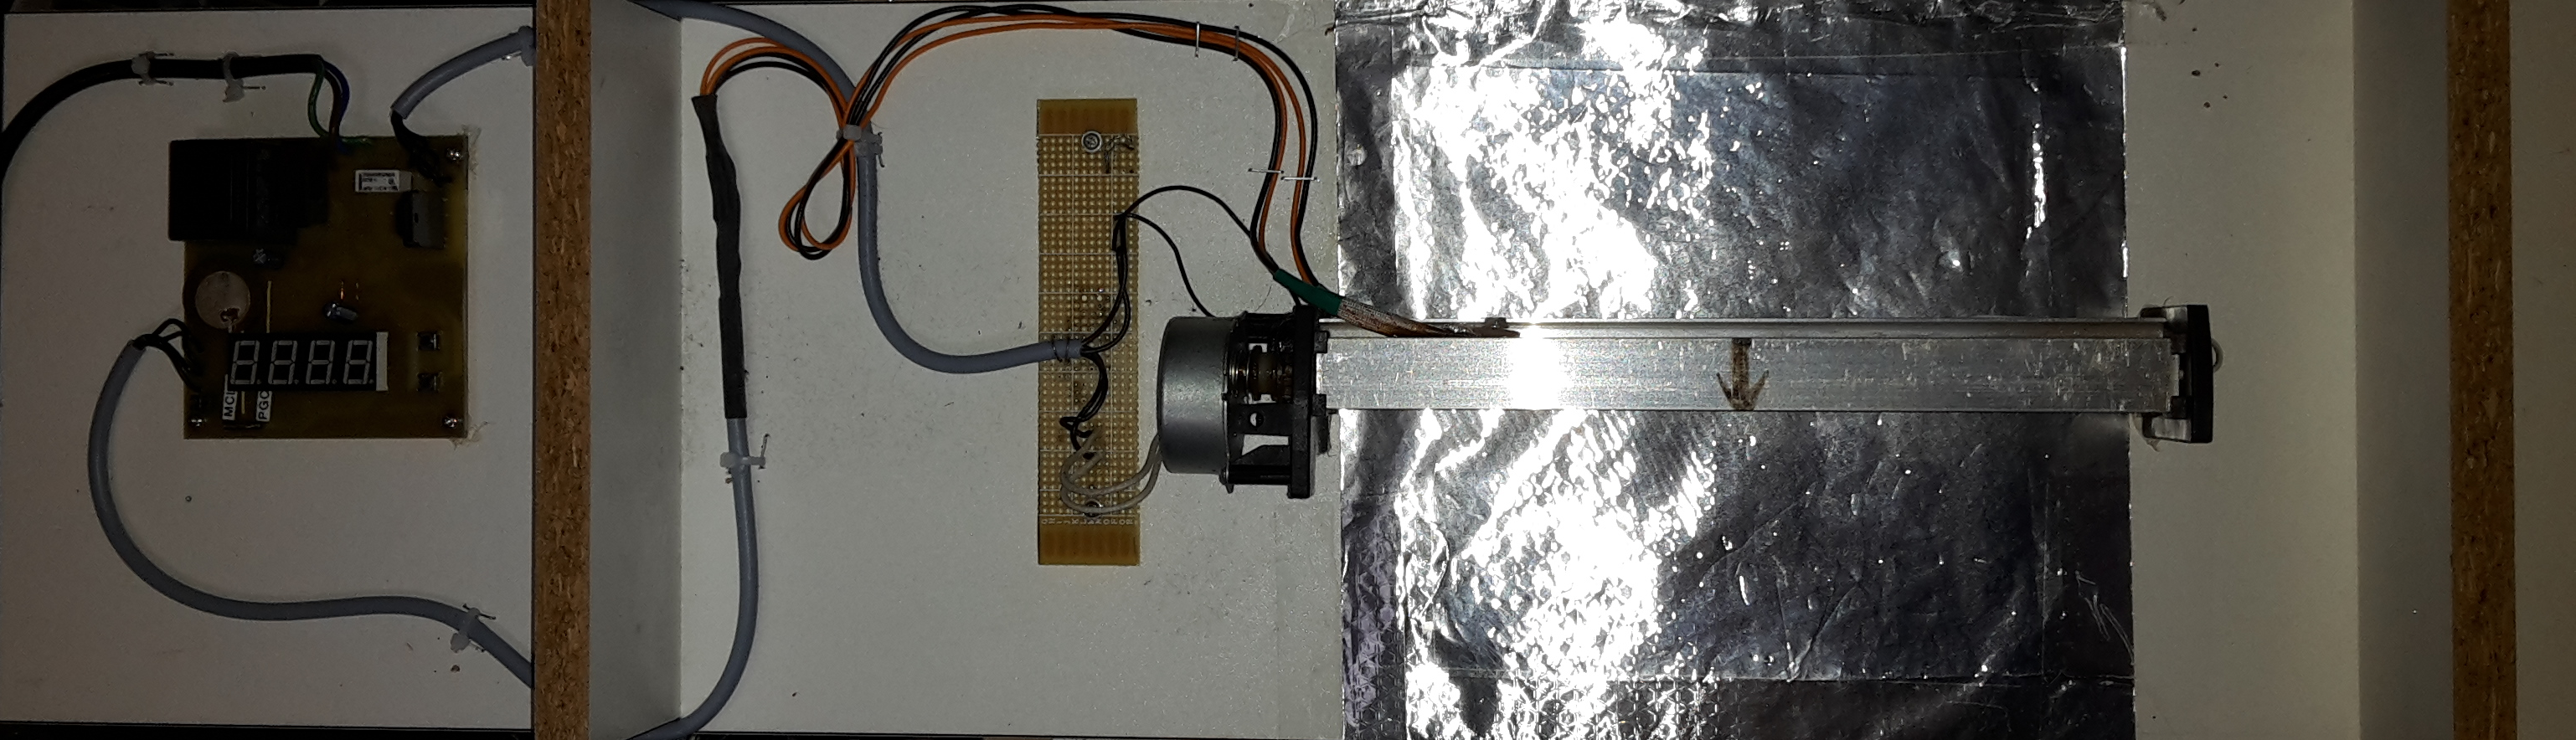
\includegraphics[width=16cm]{laminiergeraet.png}
	\centering
	\caption{Laminiergerät}
\end{figure}

%Platine 
\begin{figure}[h]
	\centering 
    \subfigure[Top-Layer]{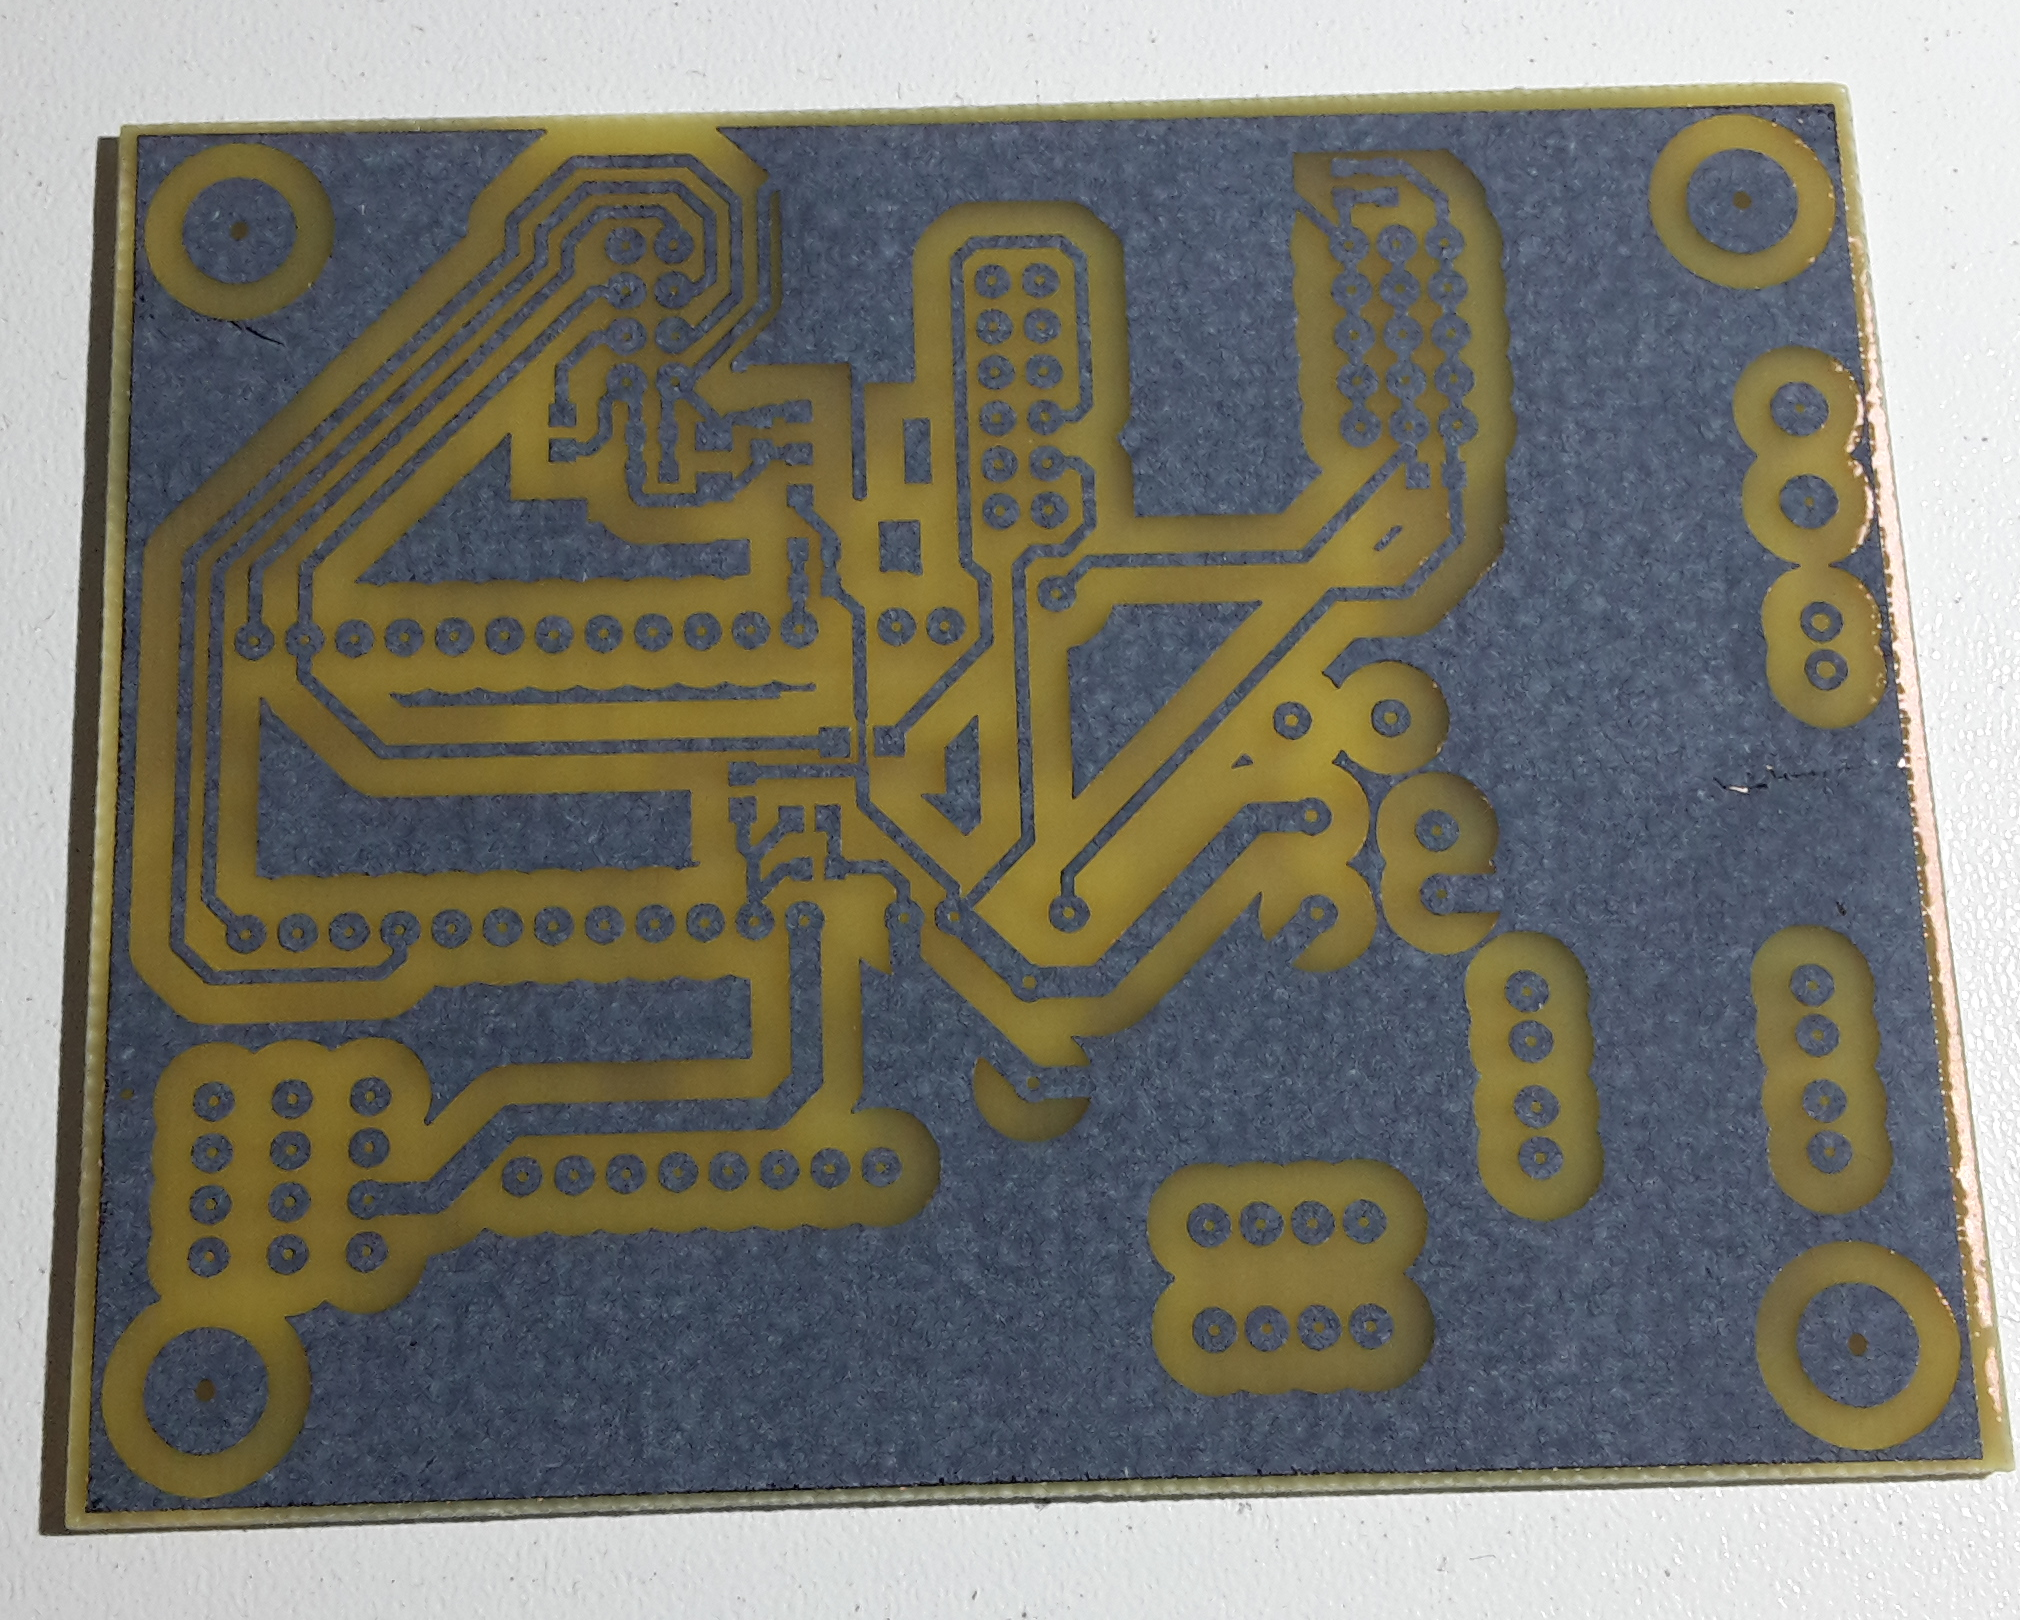
\includegraphics[width=7.5cm]{pcbTop.png}} 
    \subfigure[Bottom-Layer]{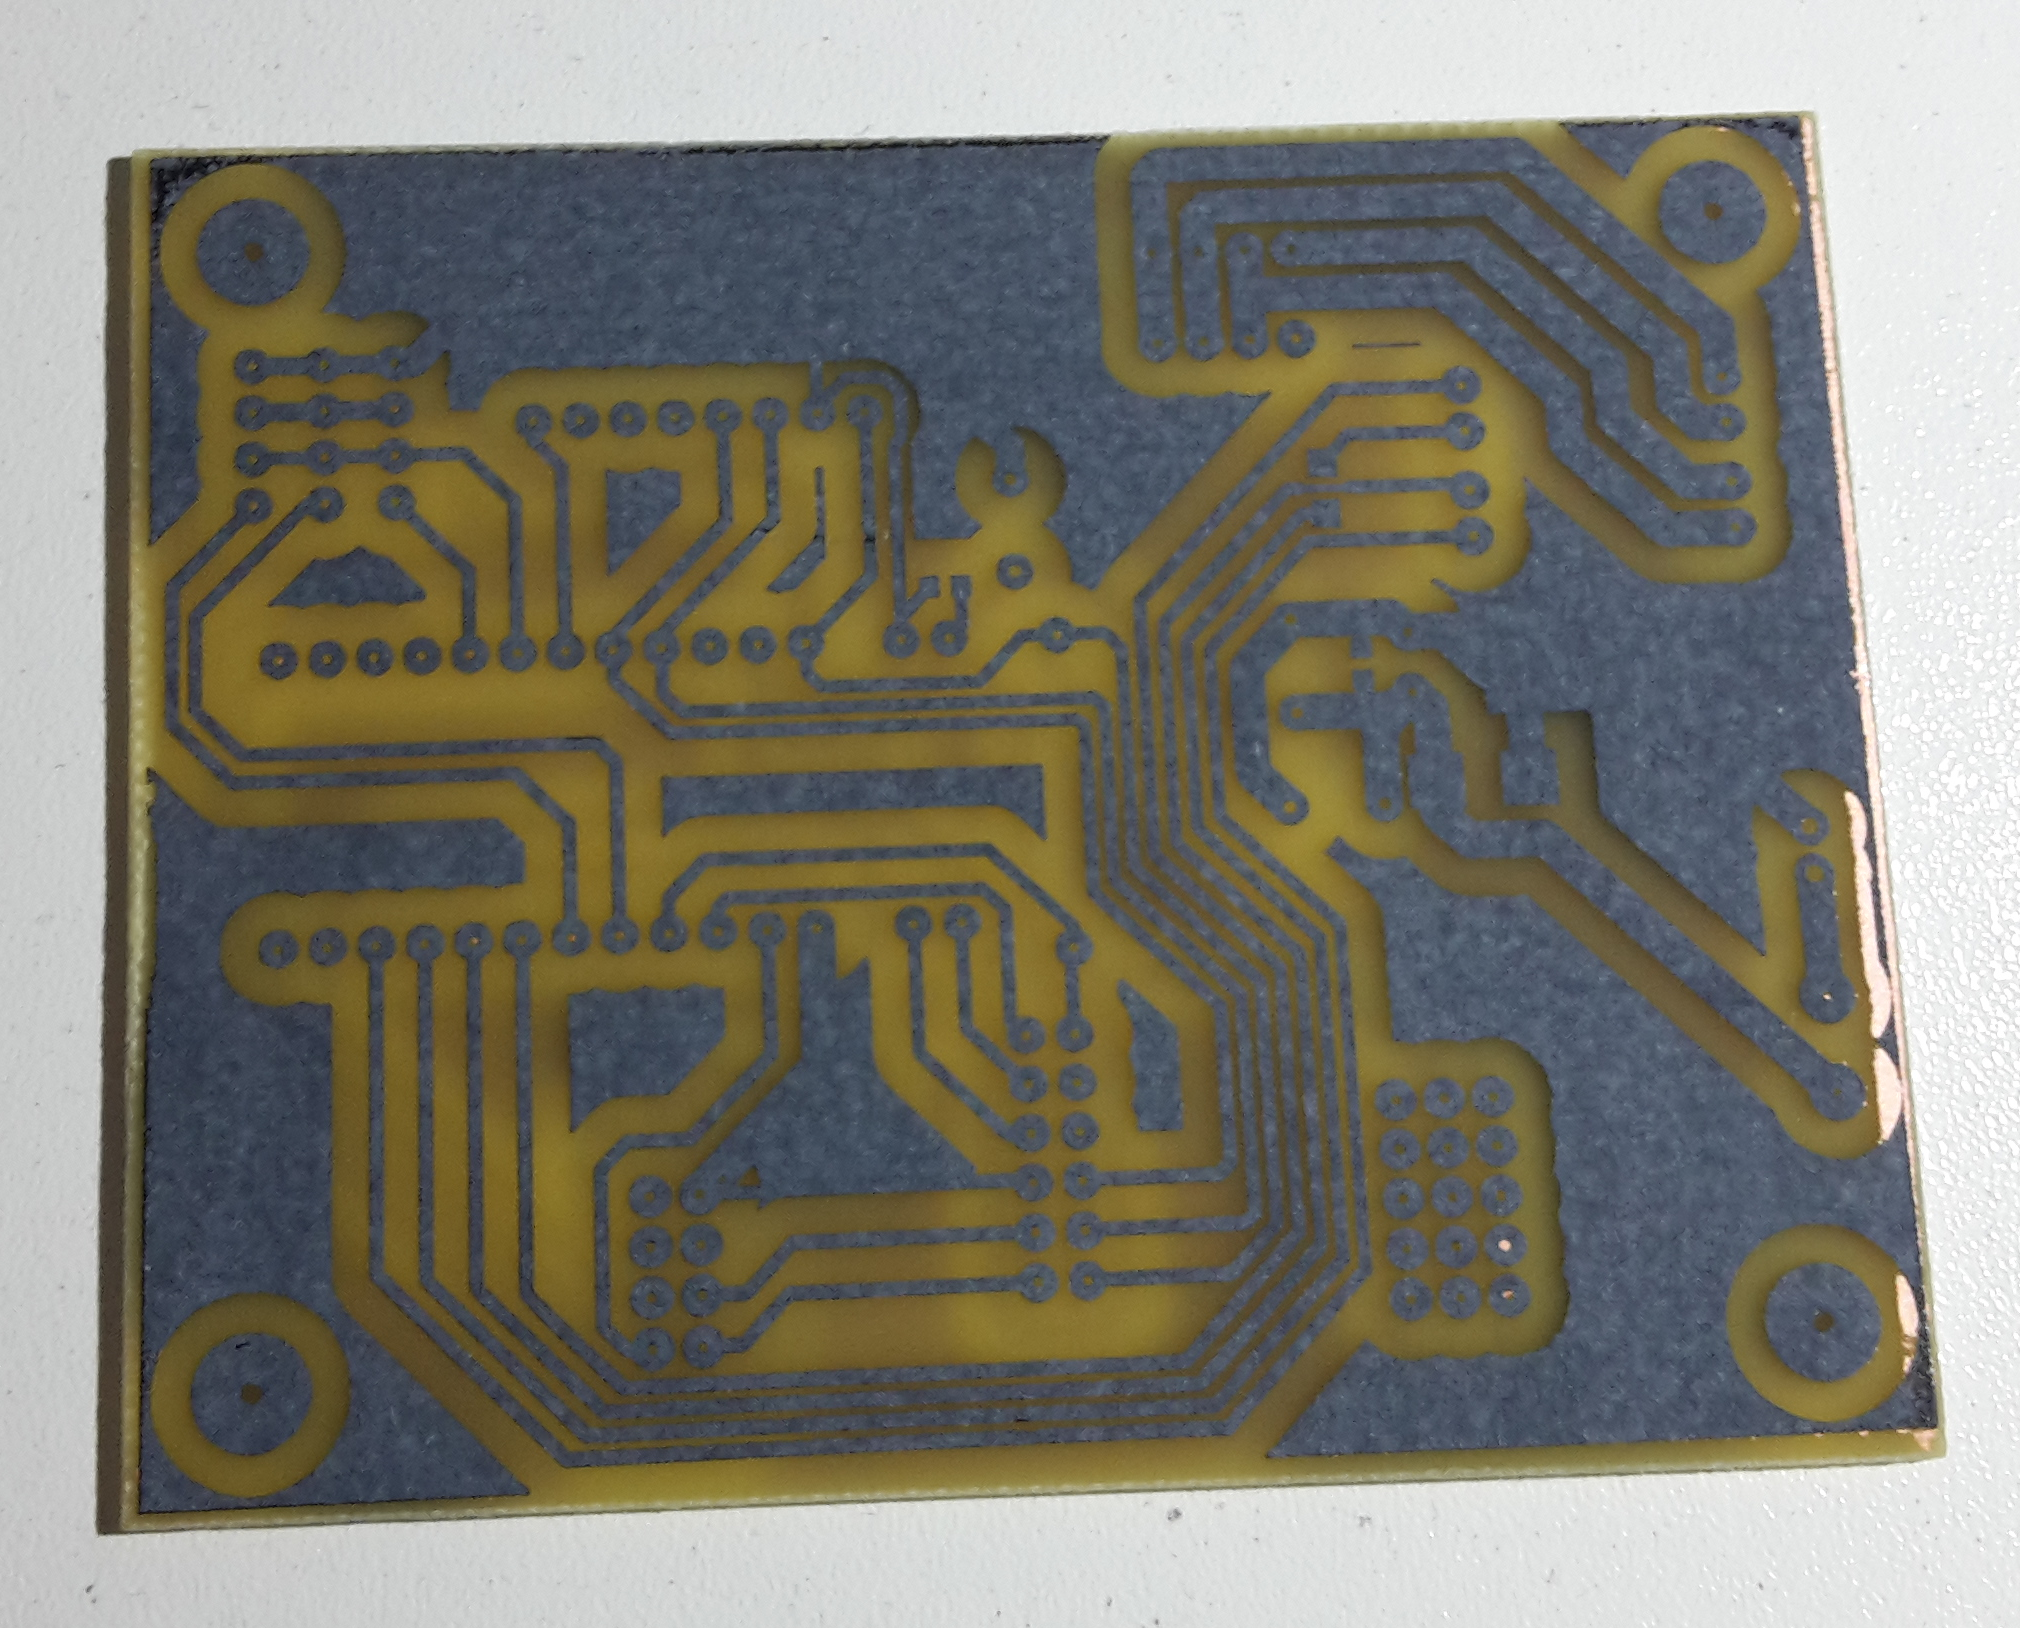
\includegraphics[width=7.5cm]{pcbBottom.png}} 
\caption{fertig geätzte Platine} 
\end{figure} 

\newpage
\subsection{Bestückung}%Yves

Zum verlöten der Komponenten kam SMD-Lot mit Bleianteil zum Einsatz.
Für SMD Komponenten wurde eine Pinzette als Hilfswerkzeug verwendet.

\subsection{Schaltung}%Yves

Die Schaltung ist relativ einfach gehalten. Im wesentlichen dient die Platine nur als Träger für die modularen Komponenten und für diverse Anschlussmöglichkeiten. Für den NRF24 wurde ein 3,3V Spannungsregler integriert.
Um etwaige Motorenwechsel zu erleichtern, sind zu deren Anschluss Federzugklemmen verbaut worden.
Wegen der Überschaubarkeit der Schaltung haben wir auf einen Schaltplan verzichtet, da das Layout selbsterklärend ist.

\newpage
\section{Fernsteuerung}%Yves

Auf die Fernsteuerung soll an dieser Stelle nicht näher eingegangen werden, da diese zum Zeitpunkt der Erstellung dieses Projektes bereits „fertig“ war.
Es wurden lediglich ein Joystick sowie ein NRF24 ergänzt.
Detaillierte Informationen finden sich im dazugehörigen Repositorium\cite{nanoGame}.

Im Rahmen eines Arduino Workshops für Anfänger entwickelte Yves Ehrlich eine Platine, welche als Shield für einen Arduino Nano fungiert. Sie enthält grundlegende Dinge wie Tasten, einen Akku, eine stabile 5V Spannungsversorgung sowie ein monochromes LCD Display mit Hintergrundbeleuchtung, um nur die wichtigsten Sachen zu nennen.

Dank der Buchsenleiste auf der Rückseite, welche neben 3,3V und 5V Spannungsversorgung auch diverse I/Os und Analogeingänge bereitstellt, lässt sich das Shield „nanoGame“ hervorragend erweitern und für viele verschiedene Dinge nutzen, so auch als Fernsteuerung für unseren Roboter.

Bei dem Joystick handelt es sich um eine Platine welche ein original Ersatzteil der Sony PSP enthält. Dieser Joystick ist sehr kompakt und ließ sich dadurch recht einfach in unsere Projekt integrieren. Es musste lediglich eine Halterung konstruiert werden, um den Joystick an das Gehäuse der Fernsteuerung zu schrauben.

Beim Funkmodul sind wir kompromissloser vorgegangen. Dieses wurde mit ein wenig Silikonklebstoff an der Oberseite fixiert.

Alle Verbindungsleitungen wurden Freiluft auf der Rückseite der Fernsteuerung zum Schacht der bereits erwähnten Buchsenleiste gelegt und dort mit Steckerleisten angeschlossen.

\begin{figure}[h]
	\includegraphics[width=12cm]{rcVorn.png}
	\centering
	\caption{Fernsteuerung vorn}
\end{figure}

\begin{figure}[h]
	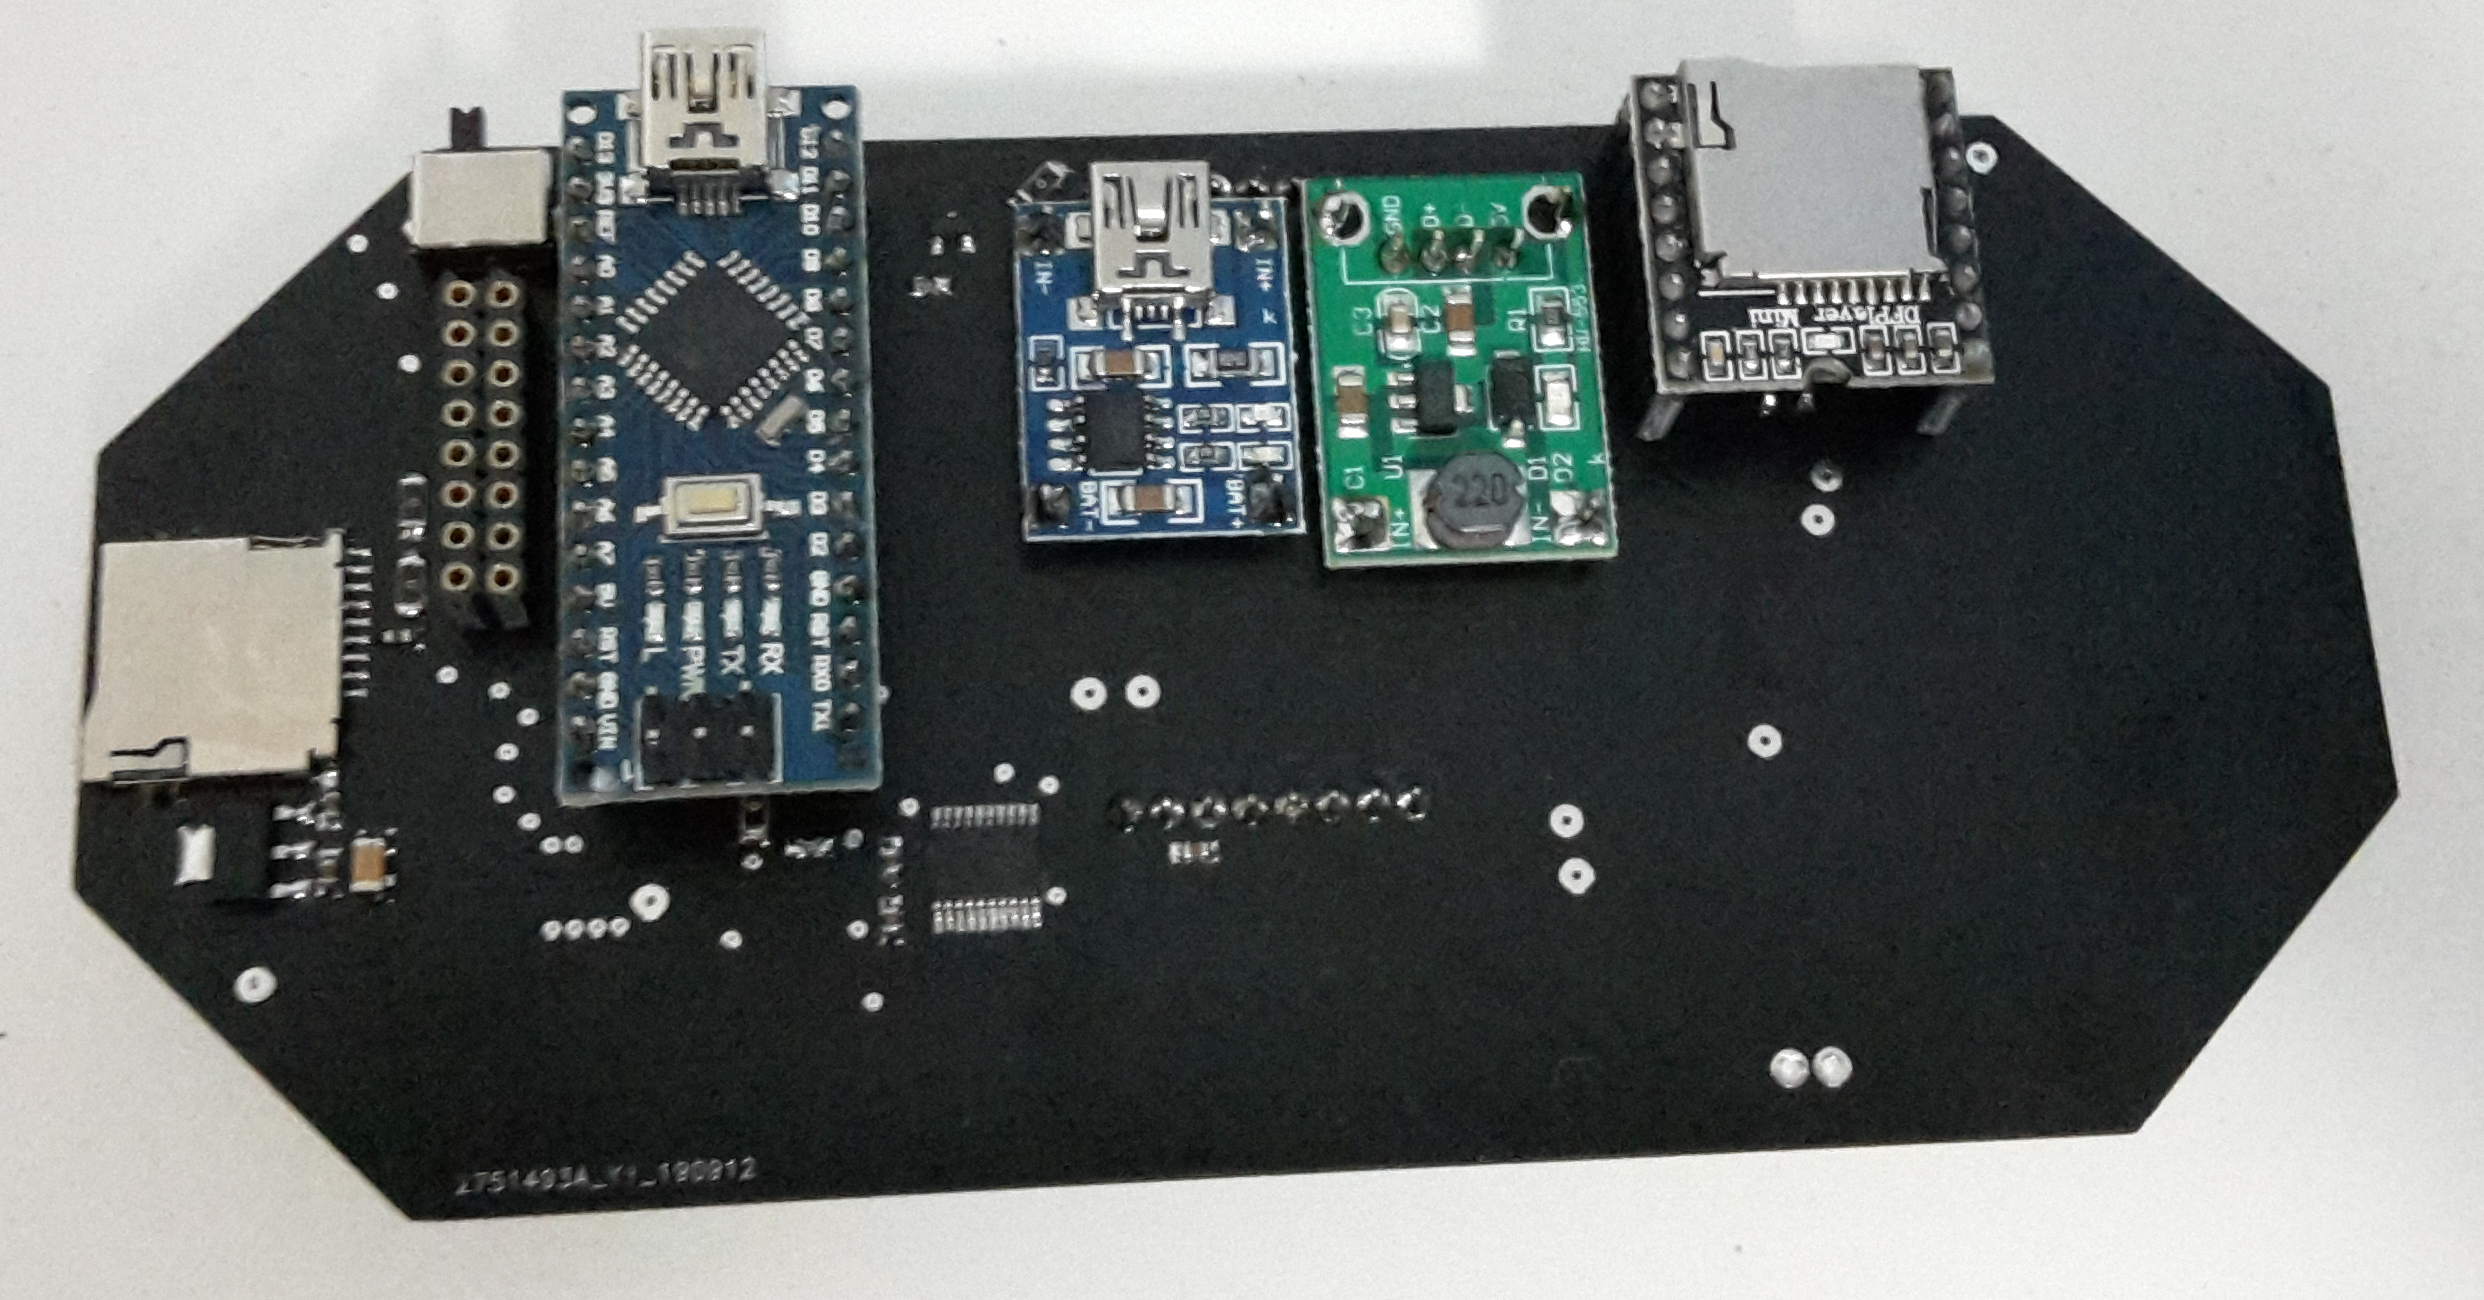
\includegraphics[width=12cm]{rcHinten.png}
	\centering
	\caption{Fernsteuerung hinten}
\end{figure}

\newpage
\section{LCD}

Als LCD kam, entsprechend dem nanoGame \cite{nanoGame} Projekt, ein monochromes Grafik-LCD mit Hintergrundbeleuchtung und einer Auflösung von 84 x 48 Pixeln zum Einsatz. Beim integrierten Controller handelt es sich um den PCD8544. Angesteuert per SPI und diversen Steuerleitungen.

Da aktuell im Projekt keine Grafiken dargestellt werden, entschieden wir uns, das LCD einfach fest in 6 Zeilen einzuteilen. Um kollisionsfrei Texte ausgeben zu können, verwendeten wir ein global deklariertes Stringarray. Jeder Teil des Codes, der etwas ausgibt schreibt in ein Element bzw. in eine Zeile. die Methode "`refreshLCD()"' liest dieses Stringarray ein und gibt die 6 Zeilen auf dem LCD aus.

\section{Code allgemein}%Yves

Um die Einsatzmöglichkeiten für den Code möglichst flexibel zu gestalten, haben wir uns bemüht, nicht blockierenden Quelltext zu schreiben.
Somit lässt sich auch mit dem recht kleinen Atmega328p bei 16 MHz Takt eine ganze Menge bewältigen.

Aktuell ist der Roboter in der Lage auf Kommandos, die er von der Fernsteuerung erhält, zu reagieren. Aus Zeitgründen konnten wir leider nur einen manuellen Fahrmodus implementieren. Dieser beinhaltet das fahren mit digitalen Tasten sowie „analog“ mit dem ergänzten Joystick.
Weiterhin implementiert wurden das erfassen von Temperaturen mit Hilfe eines DS1820 und eine Distanzmessung mit einem HC-SR04 Ultraschallsensor.

Die Übertragung von Kommandos ist relativ einfach gehalten. Das erste Byte im commands Array ist ein Kommando, gefolgt von 2 Bytes mit Daten. Diesem Muster folgend ist jedes dritte Byte ein Kommando, gefolgt von zwei Datenbytes.
Da das Array eine feste Größe von 32 Byte hat, lassen sich folglich bis zu 10 Kommandos übertragen. Wie viele Kommandos jeweils übertragen werden und in welcher Reihenfolge diese im Array vorkommen, also ob Byte 0,3,6,9...usw., spielt keine Rolle.

\newpage    
\section{SPI}%Lukas
\subsection{Was ist SPI?} %Lukas
SPI - Serial Peripheral Interface ist der Standard für ein Synchronen Seriellen Datenbus. Dieser Datenbus kann zwei digitale Schaltungen mittels Master-Slave prinzip verbinden \cite{SPI}. Der Bus ermöglicht die verwendung von Mehreren Slaves, jedoch wird die Anzahl der Slaves durch die Anzahl der CS - ChipSelect Leitungen begrenzt. Die Datenübertragung geschiet über eine Seperate Leitung, auch SD (Serial Data) genannt. 
\paragraph{Rolle des Masters}
Der Master gibt das Taktsignal über den SCK (Serial Clock) Ausgang an, desweiteren wählt er einen Slave mit welchem er kommunizieren möchte über den CS (ChipSelect).
\paragraph{Rolle des Slaves}
Der Slave ist solange inaktiv bis dieser über den CS Pin aktiviert wird. Nach der Aktivierung wird über Serial Data kommuniziert, das Taktsignal wird über den SCK Synchronisiert bzw vom Master übernommen. 

\subsection{Einsatz von SPI innerhalb des Projektes}
\paragraph{Verbindung: }
Um die Verbindung zwischen dem nRF24L01 Chip und dem Arduino herzustellen  wurden zunächst alle Verbindungen getätigt. Im Folgender Graphik ist das Pinout vom nRF24L01 Chip abgebildet. Dabei sind die Kürzel wie folgt benannt: CE - Chip Enable dieser entspricht dem Chip Select Pin, CSN -Ship Select Not dieser ist die Invertierte version des CE, SCK - Serial Clock, MISO - Master in Slave out, MOSI - Master out Slave in und die beiden Pins für die Stromversorgung VCC und Ground. Die beiden pins MISO und MOSI sind die Datenleitungen und werden an den Gleichnamingen Pins des Arduinos angeschlossen. Desweiteren ermöglicht der IRQ Interruptsteuerung dieser Pin ist Optional zu verwenden.
\begin{figure}[h]
	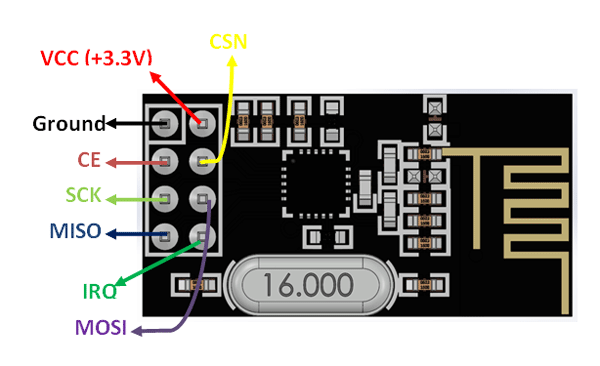
\includegraphics[width=8cm]{nRF24L01Pinout.png}
	\centering
	\caption{Pinout des nRF24L01 Chips \cite{nRF24Pinout}}
\end{figure}

\newpage
\section{Drahtlose Verbindung} %Lukas
    Wie schon zuvor erwähnt wird für die Basis der Funksteuerung das Arduino Shield verwendet, welches mit dem nRF24L01 Chip erweitert wurde. Der Roboter wurde ebenfalls mit dem nRF24L01 ausgestattet.
    \subsection{Allgemeine Verwendung von RF24} %Oder nur als paragraph je nachdem wie viel zusammen kommt.
       Die Opensoucre Bibliothek RF24 \cite{RF24Lib} diente als Codebasis für die Funksteuerung. Da diese Bibliothek bei korrekter Verwendung genau auf die Kommunikation zwischen zwei nRF24L01 Chips abgestimmt ist.
       Zur Verwendung der Bibliothek muss sie nur inkludiert und Instanziiert werden dabei werden die Beiden Pins CE und CSN für das Hardware-SPI konfiguriert.
       
       \begin{file}[RF24 initialisieren]
        \begin{lstlisting}[language=C++]
#include <RF24.h>
RF24 radio(A2, A3); // CE, CSN
const byte address[6] = "00001";
        \end{lstlisting}
        \end{file}
        
        Damit sind bereits Sämtliche Konfigurationen für die Hardware-SPI Kommunikation zwischen Arduino nano und dem nRF24L01 erledigt.
        Kommunizieren zwischen zwei dieser Setups wird dann durch die Funktionen read und wirite,
        jedoch muss vor dem Start einer Kommunikation die Methoden begin(),
        openWritingPipe(address) mit address als Kommunikationsleitung und stopListening() bei Sender bzw startListening() beim Empfänger aufgerufen werden.
        Die Methode setPALevel() setzt den Power Amplifiyer Level umso höher dieser Wert umso Stärker das Signal,
        wodurch der Stromverbrauch Steigt.
        Der Anstieg des Stromverbrauchs kann auch bei einer nicht ganz konstanten Stromversorgung dazu führen das das Modul nicht korrekt funktioniert.
       \begin{file}[RF24 initialisieren]
        \begin{lstlisting}[language=C++]
//An der Sender Seite
radio.begin();
radio.openWritingPipe(address);
radio.setPALevel(RF24_PA_MAX);
radio.stopListening();
radio.write(&payload, sizeof(payload));

//An der Empfaenger Seite
radio.begin();
radio.openReadingPipe(0, address);
radio.setPALevel(RF24_PA_MAX); 
radio.startListening();
if (radio.available()) {
	radio.read(&payload, sizeof(payload));
	//Payload weiter verarbeiten.
}
        \end{lstlisting}
        \end{file} 
	\subsection{Verwendung von RF24 innerhalb dieses Projektes}
	\paragraph{Am Anfang des Projektes: }
	Zu Begin des Projektes wurde zuerst die Funkkommunikation zwischen zwei Arduino's mittels nRF24L01 getestet, dabei gab es schon die ersten Komplikationen. Da der Chip nicht korrekt mit den Hardware SPI Anschlüssen des Arduino verbunden wurde. Nach dem weiteren Einlesen in die Funktionsweise von SPI konnten die Verbindungen richtig gesetzt und diese Komplikation wieder aufgehoben werden.
	\paragraph{Logik hinter der Kommunikation: }
	Um den Roboter mit der Fernsteuerung auch Steuern zu können musste erst ermittelt werden welche Daten der Roboter benötigt um zu fahren. Diese Daten wurden dann in ein 32Byte großes Commands Array gespeichert, welches dann übertragen wurde. Das Array besteht aus Folgenden Inhalten:
\begin{enumerate}
\item speedA      - Geschwindigkeit des rechten Motors. 
\item dirA        - Vorzeichen der Geschwindigkeit des rechten Motors.
\item speedB      - Geschwindigkeit des linken Motors.
\item dirB        - Vorzeichen der Geschwindigkeit des linken Motors.
\item goDrive     - startet autodrive.
\item stopDrive   - stoppt autodrive.
\item getTemp     - löst Temperaturübertragung aus.
\item timeToDrive - Zeit die der Roboter fahren soll.
\item nothing     - Stoppt den Roboter.
\end{enumerate}

\paragraph{Übertragung der Commands} 
Das Commands Array wurde dann wie in der Sektion allgemeine Verwendung von RF24 beschrieben Übertragen, dabei ist die Payload das Commands Array. Der Sender ist Die Fernsteuerung und der Roboter ist der Empfänger. Der Empfänger besitzt daher auch die commandInterpretation() Funktion, welche die entsprechenden Kommandos liest und umsetzt.

\newpage
\section{Steuerung} %Lukas
Der Roboter kann über ein Steuerkreuz mit 4 Buttons oder einen Joystick gesteuert werden. Begonnen wurde mit der Steuerung über die Buttons, dann wurde die Steuerung mittels Joystick realisiert und anschließend wurde diese dann noch stark variable als C++ Library Implementiert.

\subsection{Button Steuerung} %Yves/Lukas
%TODO verwendet wurde die lib ShiftRegButtons...
Die Button Steuerung ermöglicht entweder Vorwärts, Rückwärts, Links oder Rechts zu fahren. Dabei werden die Beiden Motoren mit den jeweilig maximalen PwM-Werten angesprochen, sprich sie sind entweder eingeschaltet oder abgeschaltet.
\paragraph{Logik hinter der Steuerung}
Der Roboter soll für Folgende Tasten folgende Bewegungen durchführen:
\begin{itemize}
\item Oben - vorwäts fahren
\item Unten - rückwärts fahren
\item Rechts - Drehung im Uhrzeigersinn
\item Links - Drehung gegen den Uhrzeigersinn
\end{itemize}

Realisiert wurde es folgendermaßen:
\begin{itemize}
\item vorwäts fahren - setzte PWM-Werte beider Motoren auf das Maximum
\item rückwärts fahren - setzte PWM-Werte beider Motoren auf das minimum
\item Drehung im Uhrzeigersinn - setze den PWM-Wert des rechten Motors auf das minimum und den des linken auf das maximum
\item Drehung gegen den Uhrzeigersinn - setze den PWM-Wert des rechten linken auf das minimum und den des rechten auf das maximum
\end{itemize}

\subsection{Joystick Steuerung} %Lukas
Die Steuerung über einen Joystick ermöglicht das kontrolieren über die Aussteuerung des Joysticks. Verwendet wurde ein klassischer Joystick, welcher aus dem Consolen bereich stammt.
%TODO Joysticknamen mit verlinkung auf datenblatt...
\paragraph{Grundlegende Verwendung des Joysticks}
Der Joystick besitzt zwei analoge Anschlüsse und überträt dort werte von 0 bis 511 je nach aussteuerung des Joysticks, jede Achse hat somit ihren eigenen Pin.
Die Werte der jeweiligen Achsen können dann über AnalogRead() mit dem Pin der Achse als Argument abgefragt werden.
Die Mittelstellung des Joysticks ist demnach bei 255.
\subparagraph{Mapping:}
Da der Bereich der Werte nicht zu dem der benötigten PWM- Werten passt werden diese mithilfe der map() Funktion von 0 bis 511 auf -255 bis 255 gemapt. 
Nach dem Mapping kann die Auswertung über die Richtung durchgeführt werden um dann in den entsprechenden fällen die gemappten werte als geschwindigkeit zu interpretieren.
\subparagraph{Anbringung und dessen Auswrikung auf die Steuerung}
Der Joystick wurde so an das Shield angebracht, so dass druch ein nach Vorne drücken die Achsenwerte für die Y-Achse kleiner werden und ein nach Links drücken die X-Achse ebenfalls kleiner werden. Die Aussteuerung nach Rechts folgt demnach zu einer erhöhung der Achsenwerte der X-Achse und die Aussteuerung nach unten eine erhöhung der Achsenwerte der Y-Achsen.   
\paragraph{Logik hinter der Steuerung}
Zuerst wurde die Logik der Button Steuerung übernommen, jedoch mit folgenden veränderungen. 
Vorwärtsfahren wird jetzt aktiviert, wenn der Achsenwert der Y-Achse kleiner als die Mittelstellung abzüglich einses toleranzbereiches ist.
Das Rückwärtsfahren wird aktiviert, wenn der Achsenwert der Y-Achse größer als die Mittelstellung zuzüglich eines toleranzbereiches ist.
Eine Drehung im Uhrzeigersinn wrid ausgelöst, wenn der Achsenwert der X-Achse größer als die Mittelstellung zuzüglich eines toleranzbereiches ist. Demnach wird eine Drehung gegen den Uhrzeigersinn ausgelöst, wenn der Achsenwert der X-Achse kleiner als die Mittelstellung abzüglich eines toleranzbereiches ist.
In dieser Version ist der Toleranzbereich im Code mit 20 Festgeschrieben.
\paragraph{Umsetzung der Steuerung}
Die Umsetzung ist nichts anderes als die PWM-Werte für die beiden Motoren in jedem der Steuerungsfälle zu ermitteln. Da die werte schon gemappt wurden können diese nun hier wieder verwendet werden. In der Folgenden Graphik ist zu erkennen wann welche werte gesendet werden und ab welcher Aussterung die PWM-Werte negativ bzw. positiv werden.
%TODO Graphik für die Übersetzung

\subsection{Überführung der Joystick Steuerung in eine Library} %Lukas
Hier wurde besonderes Augenmerk auf Wiederverwendbarkeit und Variabilität gelegt.
Des weiteren ist die Library komplett in C++ geschrieben. Wie genau eine C++ Library erstellt wird, wird in dieser Sektion nicht aufgefasst sondern nur die Besonderheiten betreffend der Joystick Library.
\subsection{Aufbau der Klassen}
Um eine höhere Variabilität und Wiederverwendbarkeit zu ermöglichen wurde die Library Objekt Orientiert programmiert. Dazu wurden drei Klassen Implementiert: Joystick, Motor und Steuerung.
\begin{figure}[h]
	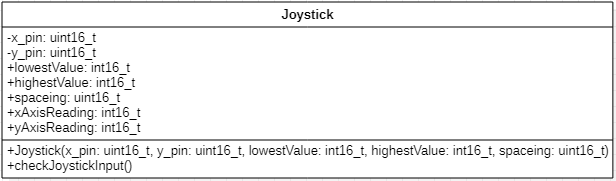
\includegraphics[width=13cm]{JoystickUML.PNG}
	\centering
	%\caption{Interpretation der Aussteuerung}
\end{figure}\begin{figure}[h]
	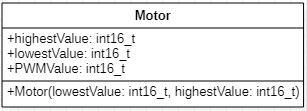
\includegraphics[width=7cm]{MotorUML.PNG}
	\centering
	%\caption{Interpretation der Aussteuerung}
\end{figure}\begin{figure}[h]
	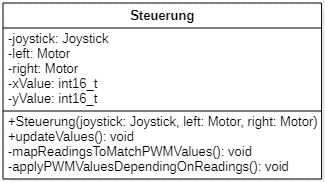
\includegraphics[width=8cm]{SteuerungUML.PNG}
	\centering
	%\caption{Interpretation der Aussteuerung}
\end{figure}
Von diesen Klassen ist die Steuerung diejenige, welche die die eigentliche Logik beinhaltet, jedoch benötigt man zur Verwendung der implementierten Steuerung zwei Motoren und einen Joystick. Um einen Motor zu erstellen reicht es den Höchsten und den Niedrigsten PWM-Wert anzugeben. Über das Attribut PWMValue lässt sich nach dem Aufruf der updateValues() Funktion der Steuerungsklasse der Aktuelle PWM-Wert jedes Motors einzeln abrufen. Beim instantiieren der Joystick-klasse müssen mehr Daten angegeben werden. Die ersten beiden Parameter legen die Pins fest an welchen die jeweilige Achse angeschlossen ist. Die nächsten zwei sind wieder der niedrige und Höchste Wert. Zum Schluss benötigt der Joystick noch einen Wert, der einen Abstand zum Mittelpunkt von der Aktivierung der Steuerung ausschließt das sogenannte spaceing. Es wird benötigt, da der Joystick selbst in der Mittelstellung werte sendet, die über bzw unter 0 liegen.    

\newpage
\section{Gedruckte Bauteile} %Yves

Alle gedruckten Bauteile haben wir selbst entworfen. einsehbar sind diese im Repositorium als STL oder aber auch unter den öffentlichen Fusion 360 Links.
\newline
%Platine 
\begin{figure}[h]
	\centering 
    \subfigure[Rahmen \cite{HC-SR04_Halterung}]{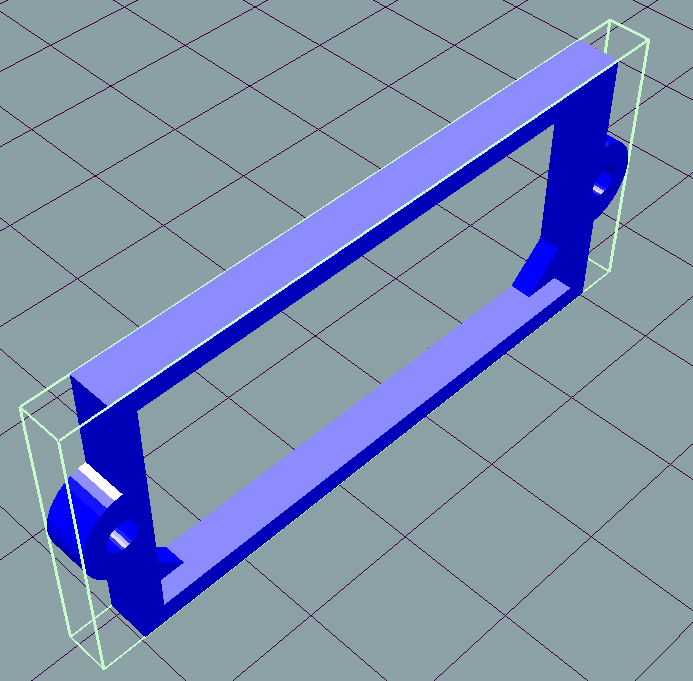
\includegraphics[width=7.5cm]{hc-sr04_rahmen.png}} 
    \subfigure[Winkel \cite{HC-SR04_Halterung}]{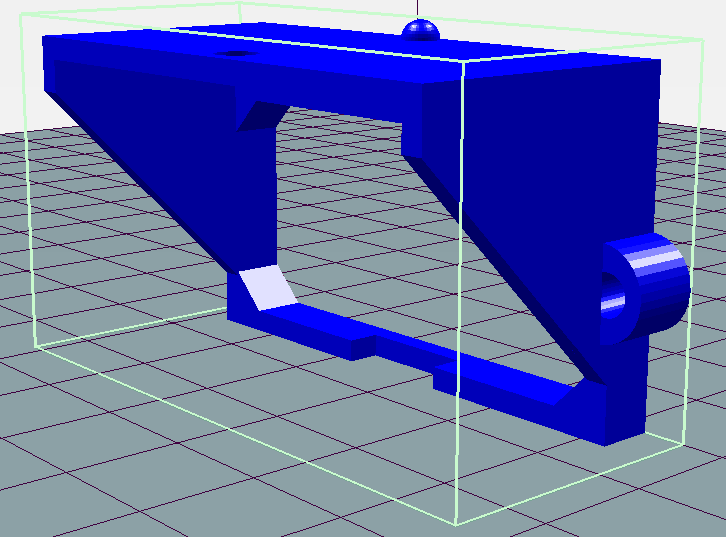
\includegraphics[width=7.5cm]{hc-sr04_winkel.png}} 
\caption{HC-SR04 Halterung} 

        \begin{minipage}[t]{0.48\textwidth}
                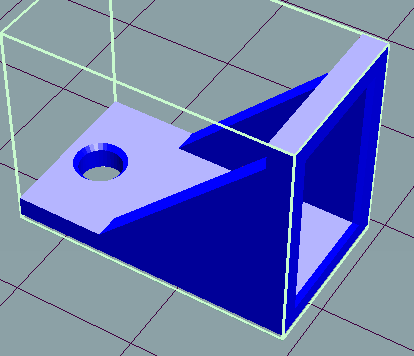
\includegraphics[width=\textwidth]{schalterhalterung.png}
                \caption{Schalterhalterung \cite{Schalterhalterung}}
        \end{minipage}\hfill
        \begin{minipage}[t]{0.48\textwidth}
                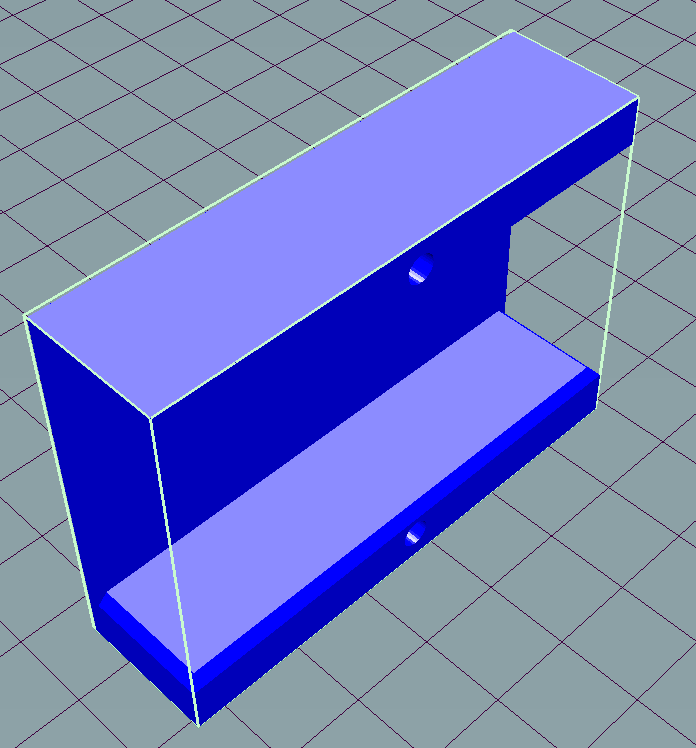
\includegraphics[width=\textwidth]{akkuhalterung.png}
                \caption{Akkuhalterung \cite{Akkuhalterung}}
        \end{minipage} 
\end{figure}


\begin{figure}
        \centering
        \begin{minipage}[t]{0.48\textwidth}
                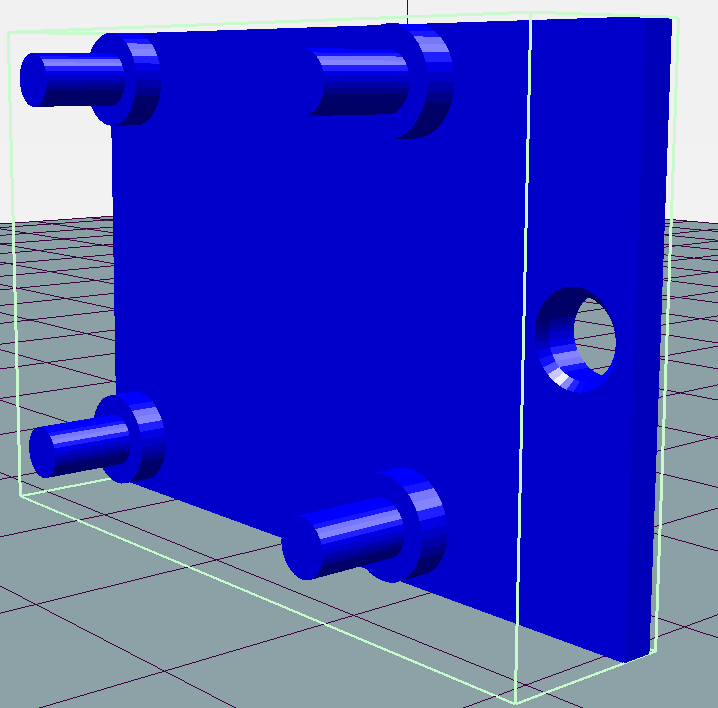
\includegraphics[width=\textwidth]{joystickhalterung.png}
                \caption{Joystick Halterung \cite{Joystick_Halterung}}
        \end{minipage}\hfill
        \begin{minipage}[t]{0.48\textwidth}
                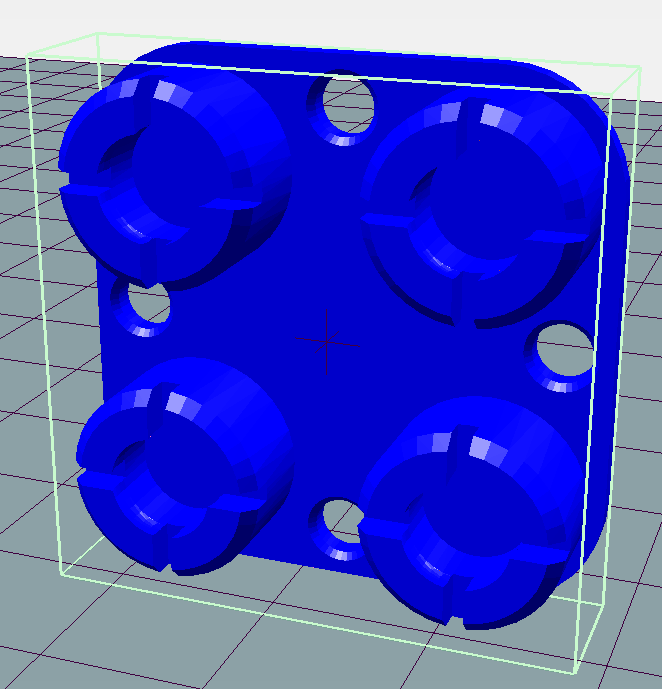
\includegraphics[width=\textwidth]{kugelrad.png}
                \caption{Kugelrad \cite{Kugelrad}}
        \end{minipage}
        \medskip

        \begin{minipage}[t]{0.48\textwidth}
                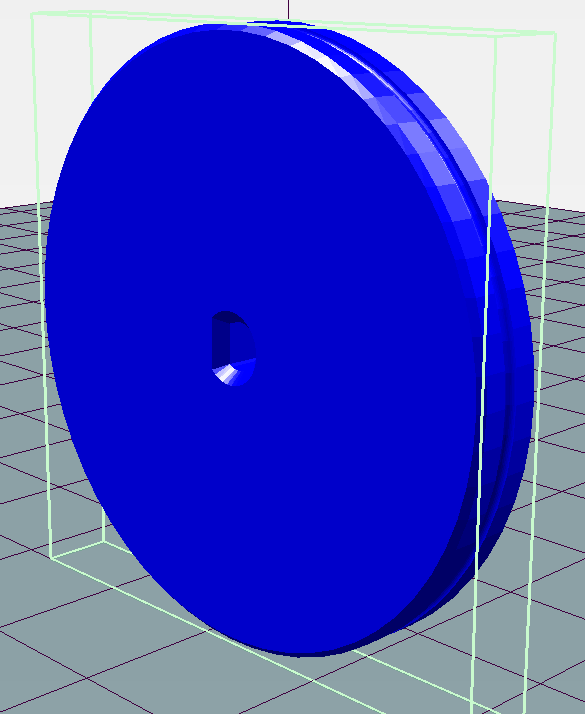
\includegraphics[width=\textwidth]{rad.png}
                \caption{Räder \cite{Raeder}}
        \end{minipage}\hfill
        \begin{minipage}[t]{0.48\textwidth}
                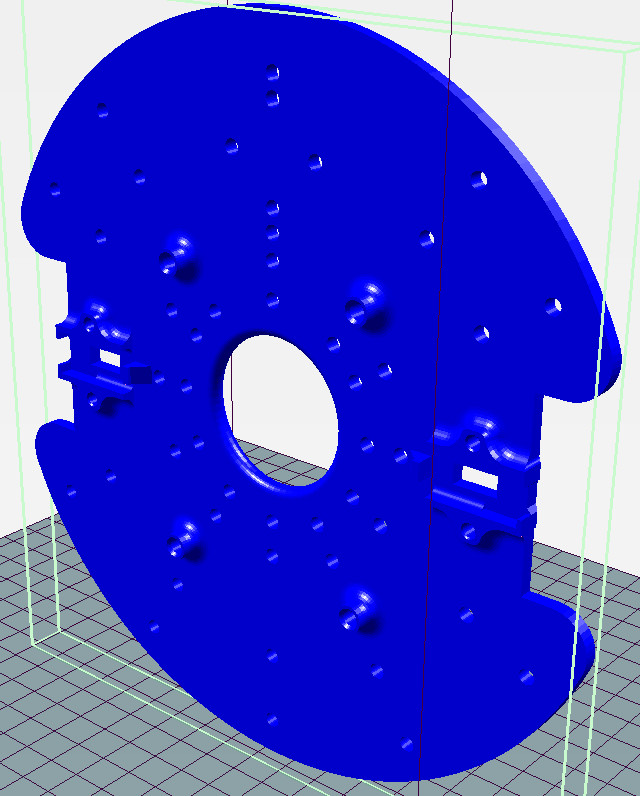
\includegraphics[width=\textwidth]{plattform.png}
                \caption{Roboter Plattform \cite{Plattform}}
        \end{minipage}
       
\end{figure}

\newpage
\section{Motorsteuerung} %Yves
\subsection{Funktionsweise eines PWM}
Die Pulsbreitenmodulation oder engl. Pulse Width Modulation (PWM) dient zur Variation der ausgegebenen Effektivspannung eines Ausgangs. Umgesetzt wird ein PWM überlicherweise mit einem Timer, welcher zählt bis er überläuft und wieder von vorn beginnt, sowie einem Komparator als auch einem Vergleichswert, welcher vorgibt, wie lang der Impuls ausgegeben werden soll. Ist der Wert vom Timer und dem PWM Sollwert identisch, so wird das Ausgangssignal abgeschalten.
Durch Variation der Impulsbreite im Verhältnis zur Periodendauer ergibt sich ein Effektivwert \ <\ = der max. Signalspannung. Das Tastverhältnis hängt von der Auflösung des Timers ab. Im Falle unseres Projektes arbeitet Timer1 als 8-Bit Timer. Somit ergibt sich ein Tastverhätnis von 1:256.
Die Grafik aus dem Atmega328p Datenblatt von Seite 133 illustriert dies noch einmal.

\begin{figure}[h]
	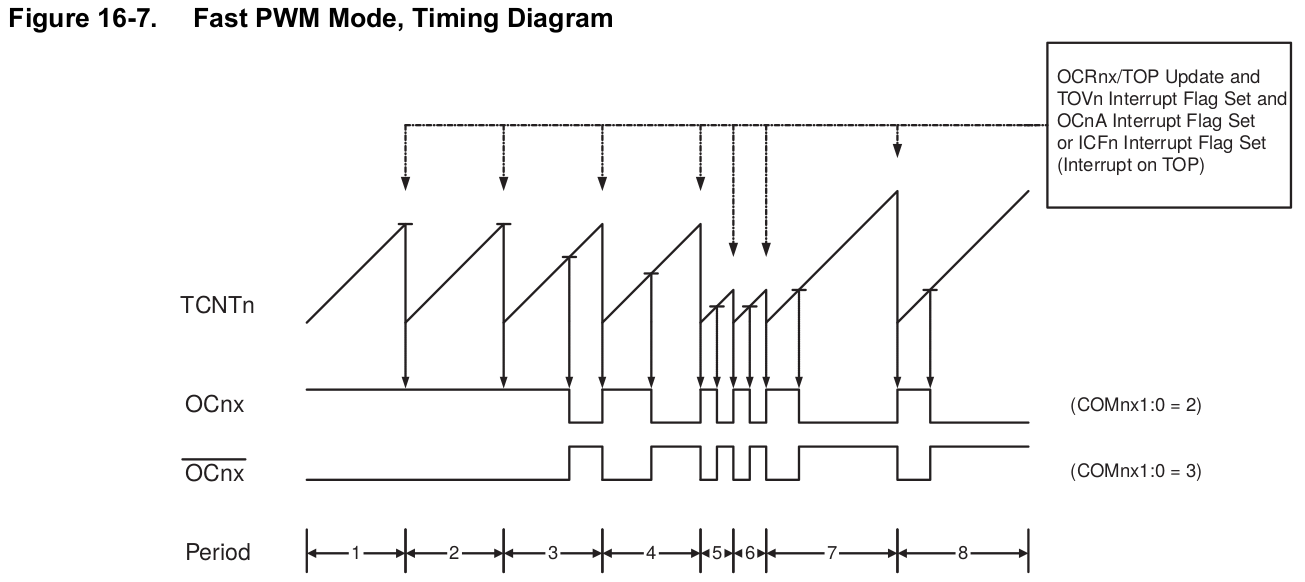
\includegraphics[width=16cm]{fastPWM.png}
	\centering
	\caption{Funktion des PWM Moduls im Atmega328p} \cite{fastPWM}
\end{figure}


\subsection{Implementierung}
Die Steuerung der Motoren wurde über den IC MX1508 realisiert. Dieser ist sehr günstig als Modul für etwa 1€ erhältlich.
Mit seinen Spezifikationen von max. 10V Versorgungsspannung und maximal 1,5A war er perfekt für dieses Projekt geeignet.
Leider konnten wir kein Datenblatt zu diesem IC finden, die Angaben stammen lediglich aus den Beschreibungen der Händler die dieses Modul verkaufen.
Es scheint sich um einen Treiber mit H-Brücke bzw. doppelter H-Brücke zu handeln, er verfügt über jeweils zwei Kanäle mit je zwei Eingängen. Je nach Polung der Eingänge kann ein Motor vorwärts oder rückwärts drehen.
Um die Geschwindigkeit der Motoren regulieren zu können schrieben wir eine Bibliothek mit dem Namen L298N (Achtung, nicht mit der gleichnamigen Bibliothek im Librarymanager der Arduino IDE zu verwechseln!).
Der Name ist angelehnt an den gleichnamigen IC, welcher dem MX1508 in seiner Ansteuerung ähnelt.
Die Bibliothek nutzt Timer1 als 8-Bit Timer für die im Atmega328p integrierten PWM-Module OC1A und OC1B.
Ein PWM Pin ist mit jeweils einem der beiden Eingangspins eines Kanals des MX1508 verbunden. Der jeweils andere Pin muss kein PWM Pin sein, muss aber je nach Drehrichtung korrekt gepolt sein. Für diese nicht-PWM-Pins haben wir die Portpins B0 (Kanal A) und D7 (Kanal B) verwendet.
\newline
Im folgenden Code ist exemplarisch zu sehen, wie das setzen eines PWM Wertes für Kanal A abläuft. Valide PWM-Werte sind -255 bis +255.


\begin{file}[MX1508]
        \begin{lstlisting}[language=C++]
 L298N::setPWM_A(int16_t pwmA) {
   if(pwmA < 0) {
     PWMA = 0xFF + pwmA;
     PORT_A |= PIN_A;
   } else {
     if(pwmA == 0) {
       PWMA = 0;
       PORT_A &= ~PIN_A;
     } else {
       PWMA = pwmA;
       PORT_A &= ~PIN_A;
     }
   }
 }
        \end{lstlisting}
\end{file}

Zunächst wird geprüft, ob der PWM-Wert "`pwmA"'  negativ ist. Davon hängt die Polung von "`PIN\_A"' ab und ob der PWM-Wert negiert werden muss.
\newline
Anschließend werden PWM-Wert und der Zustand des nicht-PWM-Pins entsprechend gesetzt.

\begin{figure}[h]
	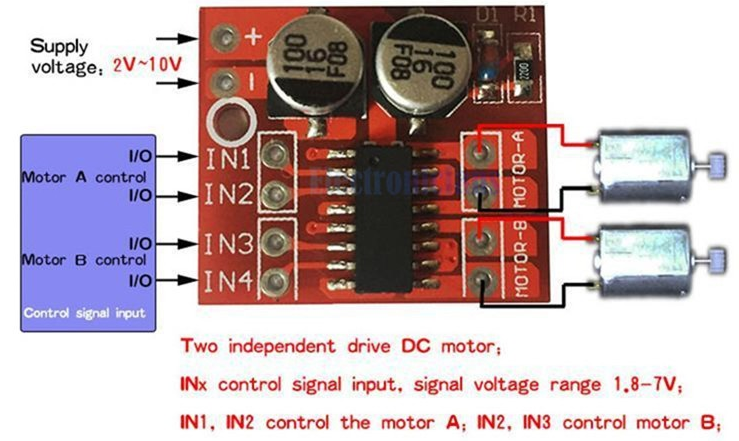
\includegraphics[width=12cm]{MX1508.png}
	\centering
	\caption{MX1508 Anschluss \cite{MX1508}}
\end{figure} 


%Folgende beiden ließen sich auch durch subsections mittels sensoric als section realisieren, kommt aber auf die menge des textes an subsections sollten nicht über eine halbe seite lang sein.
\newpage
\section{Thermosensor} %Nick
\subsection{OneWire}
OneWire ist eine serielle Schnittstelle, die nur mit einer Datenleitung auskommt. Jedes angeschlossene Gerät hat eine eigene 64bit ROM Adresse, die man gezielt ansprechen kann. Alternativ, kann man Befehle an alle Geräte senden indem man den Skip ROM-Command (0xCC) benutzt. Anschließend kommt der eigentliche Befehl mit write(), der ausgeführt werden soll. Danach werden die Daten auf ein Scratchpad-Speicher geschrieben von wo sie per read() gelesen werden können.
\subsection{Sensor und dessen Integration}
Wie bereits erwähnt benutzen wir einen Dallas DS18b20  1-Wire Digital Thermometer, um die Motortemperatur zu messen. Der DS18b20 speichert die Temperatur als einen 9bit - 12bit Wert und kann Temperaturen im Bereich von -55°C bis 125°C messen. Für unsere Bedürfnisse reicht es wenn wir in 1-er Schritten messen. Der Sensor kommt aber auch mit kleineren Inkrementen zu recht. Der Sensor benötigt die OneWire-Library um angesprochen zu werden.\\
\begin{figure}[h]
	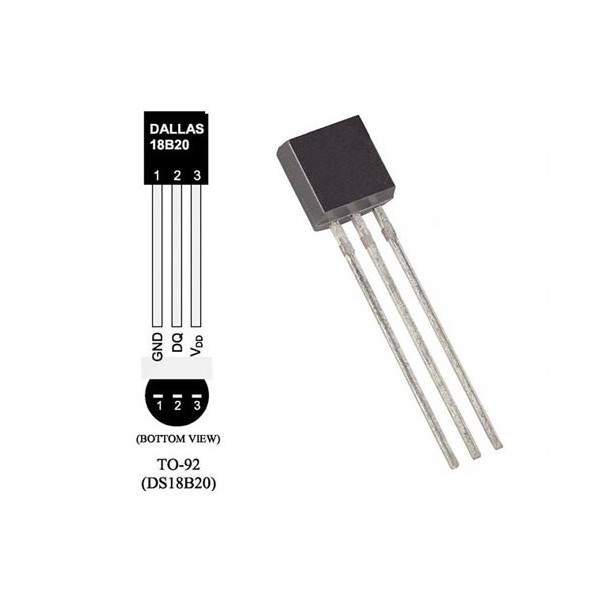
\includegraphics[width=12cm]{ds18b20.jpg}
	\centering
	\caption{Der benutzte Sensor \\1) Erdung 2) Datenleitung 3) Spannung}
\end{figure}
\\
Eine Messung wird durchgeführt indem der Sensor Takte, innerhalb eines Zeitfensters zählt. Der Zähler startet bei einem Wert, der -55°C darstellt. Erreicht der Zähler 0 schneller als das vorgegebene Zeitfenster wird das Temperaturregister inkrementiert. Der Zähler wird dann auf einen vom Slope Accumulator Circuitry abhängigen wert gestellt und wieder runtergezählt. Dies wiederholt sich solange bis das festgelegte Zeitfenster abgelaufen ist. \\
\\
Es gibt verschiedene Wege den Code für den Sensor zu implementieren. Der einfachste Weg wäre die DallasTemperature-Library zu benutzen.

\begin{file}[DS18B20]
        \begin{lstlisting}[language=C++]
#include <OneWire.h>
#include <DallasTemperature.h>
		
OneWire oneWire(x);
DallasTemperatures sensors(&oneWire);

void setup(){
  Serial.begin(9600);	
  // Die Library starten
  sensors.begin();
}

void loop(){
  // Temperaturmessung anfordern
  sensors.requestTemperatures();	
  // Temperatur anzeigen
  Serial.print(sensors.getTempCByIndex(y));
  
}

        \end{lstlisting}
\end{file}
OneWire wird auf Pin 4 initialisiert, dann wird OneWire an sensors() übergeben. Damit weiß die Library wo der Sensor angeschlossen ist. Mit sensors.begin() startet man die Library. Eine Messung fordert man mit requestTemperatures() an und mit getTempCByIndex(y) kann man einen bestimmten Sensor, wenn man mehrere hat, nach der Temperatur in Grad Celsius abfragen. Mit der Library ist das ganze also sehr einfach.\\
\\
Das war auch der erste Ansatz. Der Clue an der Sache ist jedoch, dass die Prozedur auf die Weise etwa 600ms dauert und das den Roboter viel zu lange blockieren würde, da er in der Zeit keine weiteren Befehle verarbeiten kann. Also wurde diese Idee mitsamt der Library gestrichen und nach einer effizienteren Alternative gesucht.\\
\\ 
Für unsere Implementierung haben wir uns an\\ \url{https://www.scargill.net/reading-dallas-ds18b20-chips-quickly/} orientiert. Dieses Beispiel ermöglicht es eine Messung in nur 5ms durchzuführen. Es wurden jedoch einige Änderungen in der Umrechnung der Temperatur gemacht. Da ein Einsatz in negativen Temperaturen nicht vorgesehen ist, machen wir eine viel simplere Umrechnung als die im Blog. \\
\\


\begin{file}[DS18B20]	
        \begin{lstlisting}[language=C++, inputencoding={utf8}, extendedchars=false]        
#include <OneWire.h>

int16_t dallas(int x){
  // Initialisiergung
  OneWire ds(x); 
  byte data[2];
  int16_t result = 0;
  // Auf Scratchpad schreiben
  ds.reset(); 
  ds.write(0xCC);
  ds.write(0xBE); 
  // Vom Scratchpad lesen
  for(int i = 0; i < 2; i++){
    data[i] = ds.read();
  } 
  result = (data[1]<<8)|data[0];
  result = result/16;
  // Messen
  ds.reset();
  ds.write(0xCC);  
  ds.write(0x44, 1);
  return result;
}
        \end{lstlisting}
        
\end{file}
Wir initialsieren im Beipspiel OneWire auf einen beliebigen Pin und setzen den Sensor mit reset() zurück. Die ROM Adresse wird dabei mit write(0xCC) übersprungen, da wir nur einen Temperatursensor haben und es somit reicht, dass wir alle Geräte auf dieser OneWire-Verbindung ansprechen.Mit write(0xBE) wird dem Sensor gesagt, dass er die Werte auf dem Scratchpad speichern soll, die wir dann mit read() in einen Array einlesen. Die Werte im Array führen wir dann zusammen und teilen sie durch 16. Die 16 ergibt sich aus einer Tabelle aus dem Datenblatt. Bei genauerer Betrachtung stellt man Fest, dass die Temperatur Werte über 0 einfach nur die Binärwerte geteilt durch 16 sind. da es für unsere Bedürfnisse genügt, dass wir nur die positiven Werte messen, belassen wir es bei dieser einfachen Umrechnung. Dann wird der Chip wieder resetet, die Addresierung übersprungen  und mit write(0x44) eine Messung durchgeführt. Es empfiehlt sich in der setup() Funktion die dallas() Funtion aufzurufen, damit er in der loop() den richtigen Wert erhält.\\
\\   
Um den Roboter so wenig wie möglich zu belasten und somit eine eine schnelle Reaktionszeit zu ermöglichen, wird die Temperaturmessung nur alle 100ms durchgeführt und nur jede Sekunde durch den Funkcontroller abgefragt. Die Abfrage wird, aus Übersichtsgründen, abseits der Steuerung gemacht.

\newpage
\section{Ultraschallsensor} %Nick
Zur Messung der Distanz zu einem Objekt vor dem Robotor benutzen wir einen HC-SR04 Ultraschallsensor. Dieser kann einen Abstant bis ca 450cm messen. Das ganze funktioniert, durch ein Signal, das der Sensor von sich gibt und die Zeit zählt bis er ein Echo zurückbekommt.\\
\begin{figure}[h]
	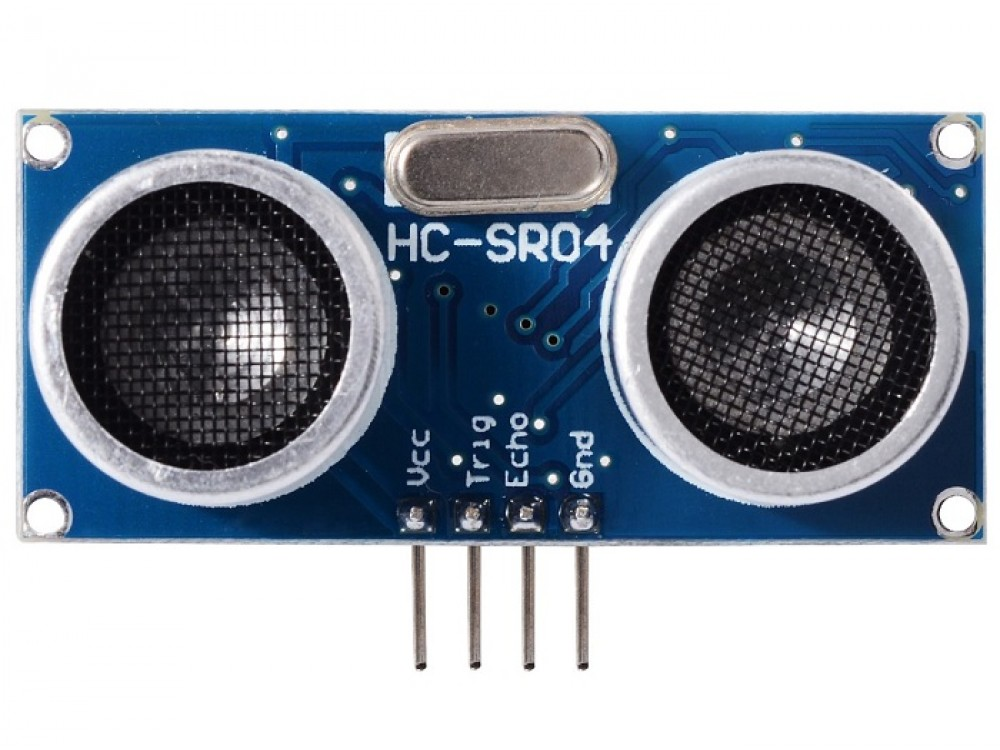
\includegraphics[width=12cm]{HC-SR04.jpg}
	\centering
	\caption{Der benutzte Sensor \\1) Spannung 2) Trigger Pin 3) Echo Pin 4) Erdung}
\end{figure} 
\\
Die Implementation ist relativ einfach. Wir setzen den Trigger Pin als Ausgang und den Echo Pin als Eingang. Wir senden mit dem Trigger Pin, dann ein Signal, welches vom Echo Pin empfangen wird und rechnen dann die Zeit die dafür gebraucht wurde in cm um.\\
\\
Zum Empfangen des Echo nutzen wir einen Pinchange Interrupt. Diese ISR wird ausgeführt, wenn ein Signal an einen bestimmten Pin kommt. Dazu aktivieren wir die nötigen PCINTs im PCIRC Register und PCMSK2 das bit für unseren Pin.\\
\\
In der ISR messen wir die Zeit bis ein Echo ankommt und teilen es, wie im Datenblatt beschrieben, durch 58 um die Distanz in Centimetern zu bekommen.

\begin{file}[HC-SR04]
		
        \begin{lstlisting}[language=C++, inputencoding={utf8}, extendedchars=false]   
int trig;
int echo;
//ISR for PCINT2
ISR(PCINT2_vect) {
  if((PIND & 64) > 0) {
    pulseStart = micros();
  } else {
    startNewMeasurement = true;
    pulseLength = micros() - pulseStart;
    newResult = true;
  }
  PCIFR = 0;
}

void measureDistance(){   
    digitalWrite(trig, HIGH);
    // ... wait for 10 µs ...
    delayMicroseconds(10);
    // ... put the trigger down ...    
    digitalWrite(trig, LOW);     
    //Serial.println("messe...");
    startNewMeasurement = false;    
}
        \end{lstlisting}
        
\end{file}
In einer setup() Funktion müssen wir den Trigger Pin als Ausgang und den Echo Pin als Eingang definieren und ein initiales Sigal mit dem trigger Pin senden. Im Anschluss aktivieren wir die nötigen Bits im PCICR und PCMSK2 Register um den Pinchange Interrupt für unseren Echo Pin zu aktivieren.\\
\\
Die measureDistance() Funktion, leitet die Messung ein. Sie gibt aus dem Trigger mit digitalWrite(trig, HIGH) Pin ein Signal an den Sensor, der dann ein Ultraschallsignal von sich für 10 Mikrosekunden abgibt, welches mit digitalWrite(trig, LOW) wieder abgestellt wird. Die ISR führt dann die eigentliche Messung durch. Da die ISR bei Anfang und bei Ende des Signals aufgerufen wird, haben wir eine Fallunterscheidung eingebaut die zu Beginn des Signals die Startzeit speichert und am Ende des Signals, daraus die Pulslänge berechnet, mit der wir die Distanz bestimmen können. Dazu müssen wir die Pulslänge, wie im bereits erwähnt, durch 58 teilen.\\
\\
Mit der Distanz die wir nun haben können wir den Roboter stoppen lassen, wenn er zu nah an einen Gegenstand ranfährt. Ihn aber komplett zu stoppen wäre unsinnig, da er sich überhaupt nicht mehr bewegen könnte. Also gucken wir nach den Motorgeschwindigkeiten und setzen diese nur auf 0 wenn sie mit einer Vorwärtsbewegung übereinstimmen. Somit kann sich unser Roboter immer noch auf der Stelle drehen oder rückwärts fahren um das Hindernis zu umgehen. 

\newpage
%----------------------------------------------------------------------------------------
%	BIBLIOGRAPHY
%----------------------------------------------------------------------------------------

\bibliographystyle{unsrt}

\bibliography{references.bib}

%----------------------------------------------------------------------------------------



\end{document}

